\chapter{Figuras} \label{Appendix:Figures}

%% INCEPTION-RESNET-V2 MODULES

\begin{figure}
    \centering
    \begin{subfigure}[t]{.45\textwidth}
      \centering
      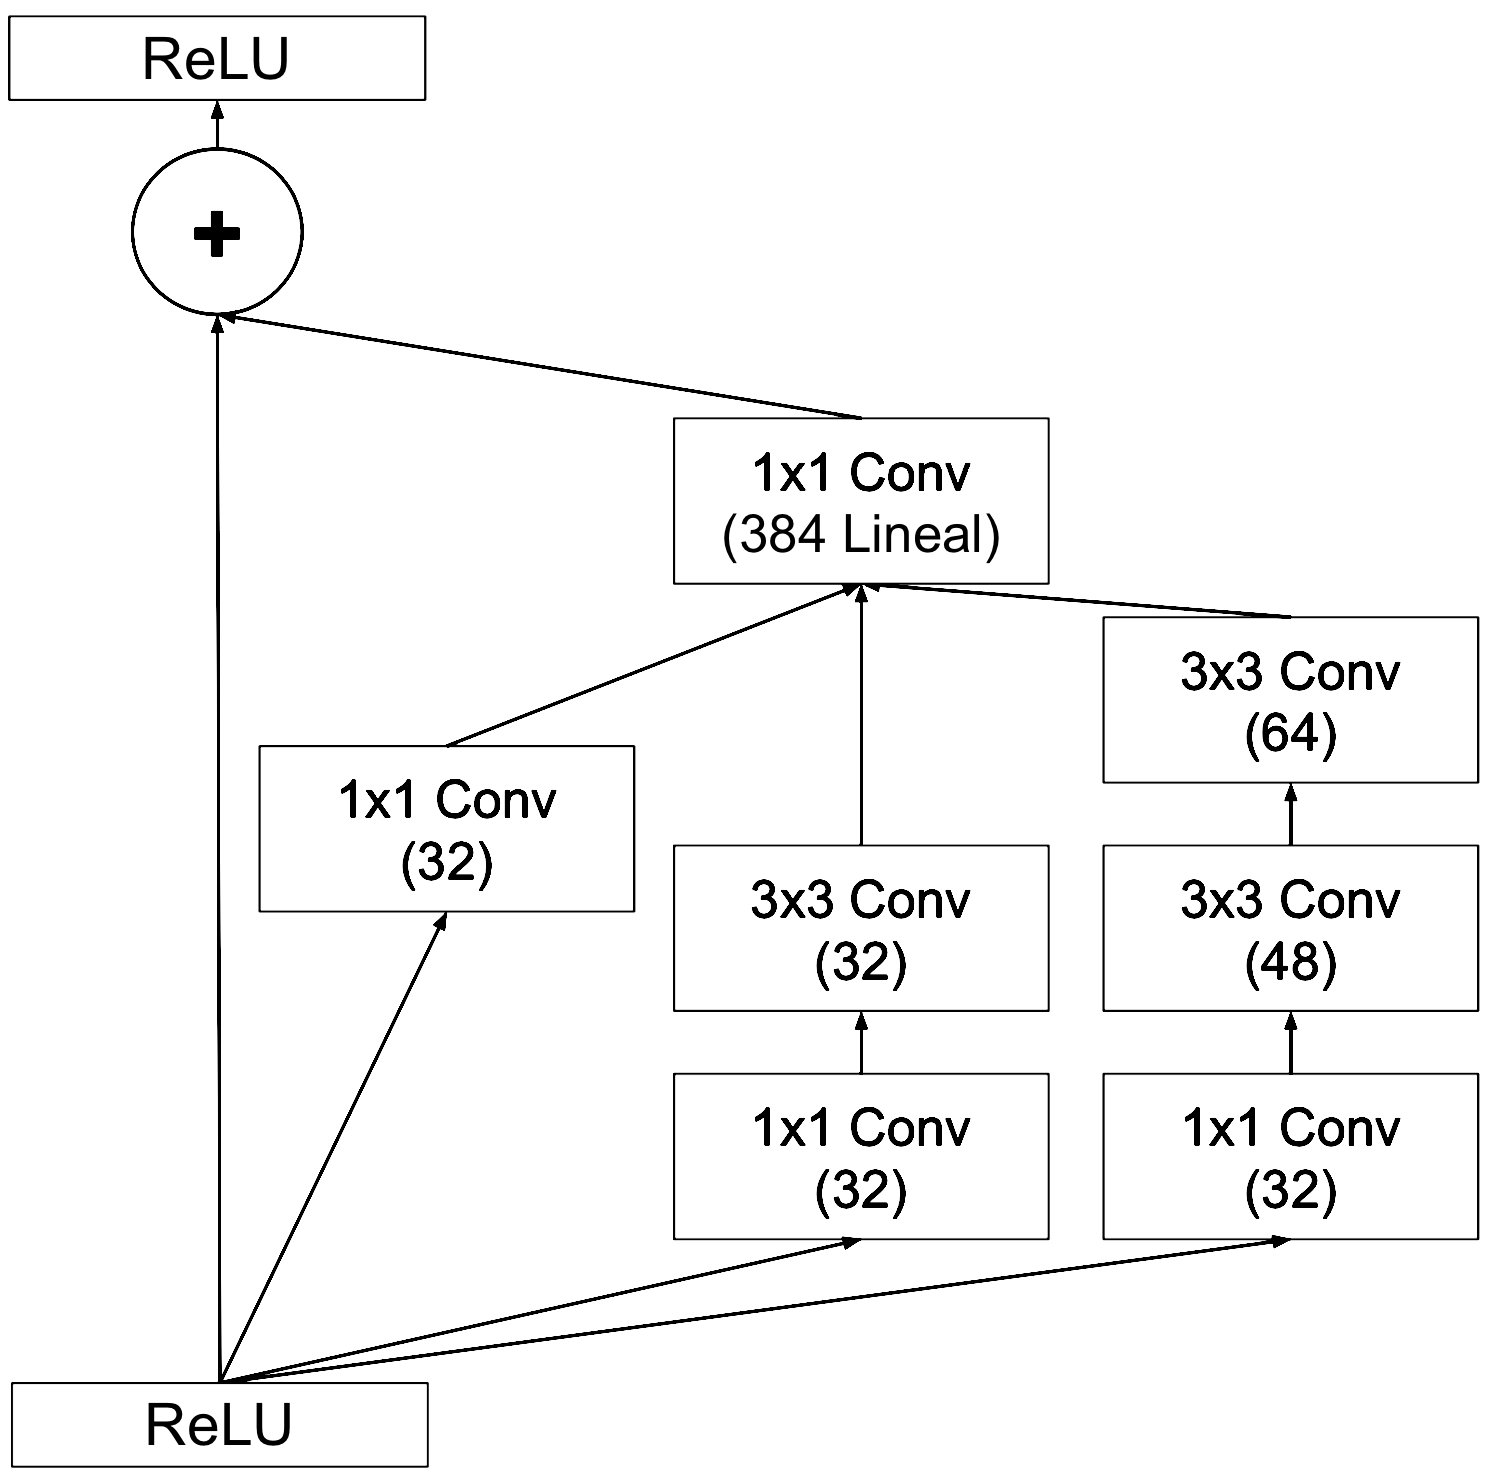
\includegraphics[width=.8\linewidth]{Images/Inception-ResNet-A.png}
      \caption{Bloque Inception-ResNet-A.}
      \label{fig:Inception-ResNet-A}
    \end{subfigure}
    \hfill
    \begin{subfigure}[t]{.45\textwidth}
      \centering
      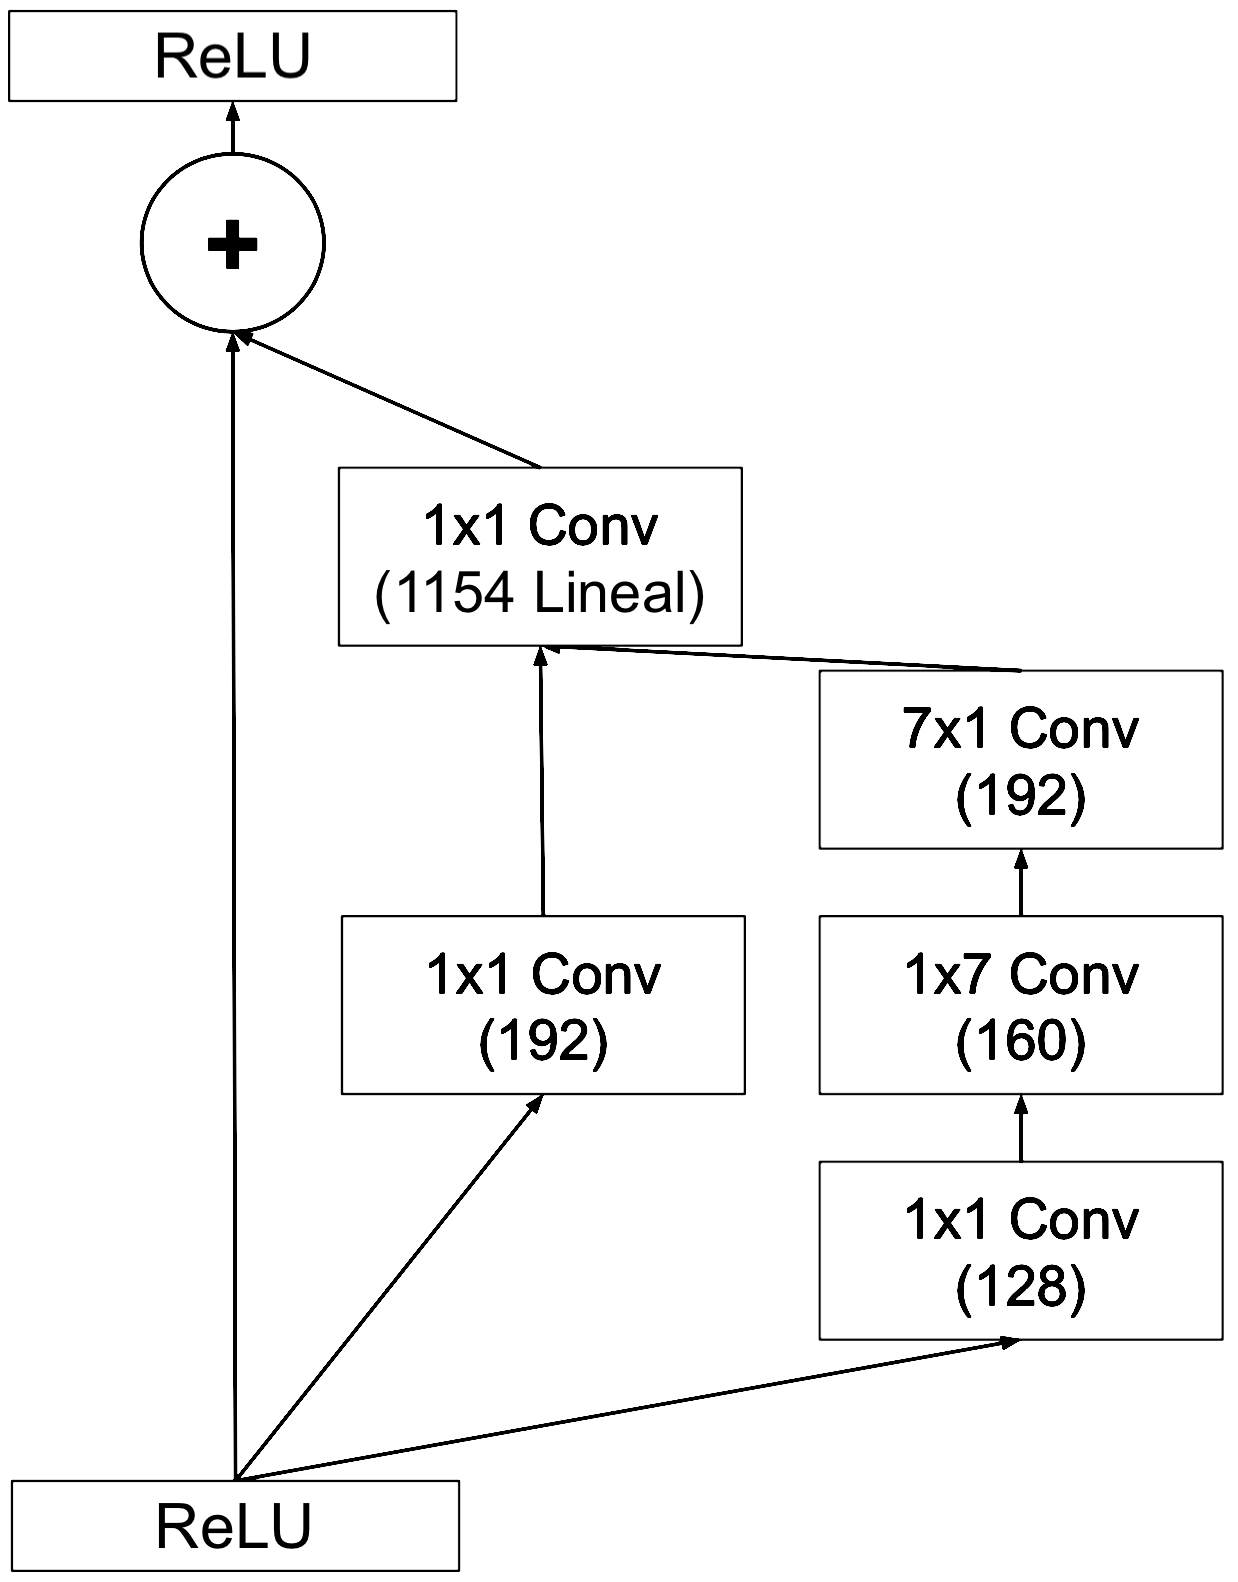
\includegraphics[width=.8\linewidth]{Images/Inception-ResNet-B.png}
      \caption{Bloque Inception-ResNet-B.}
      \label{fig:Inception-ResNet-B}
    \end{subfigure}
    
    \vspace{1cm}
    \begin{subfigure}[t]{.45\textwidth}
      \centering
      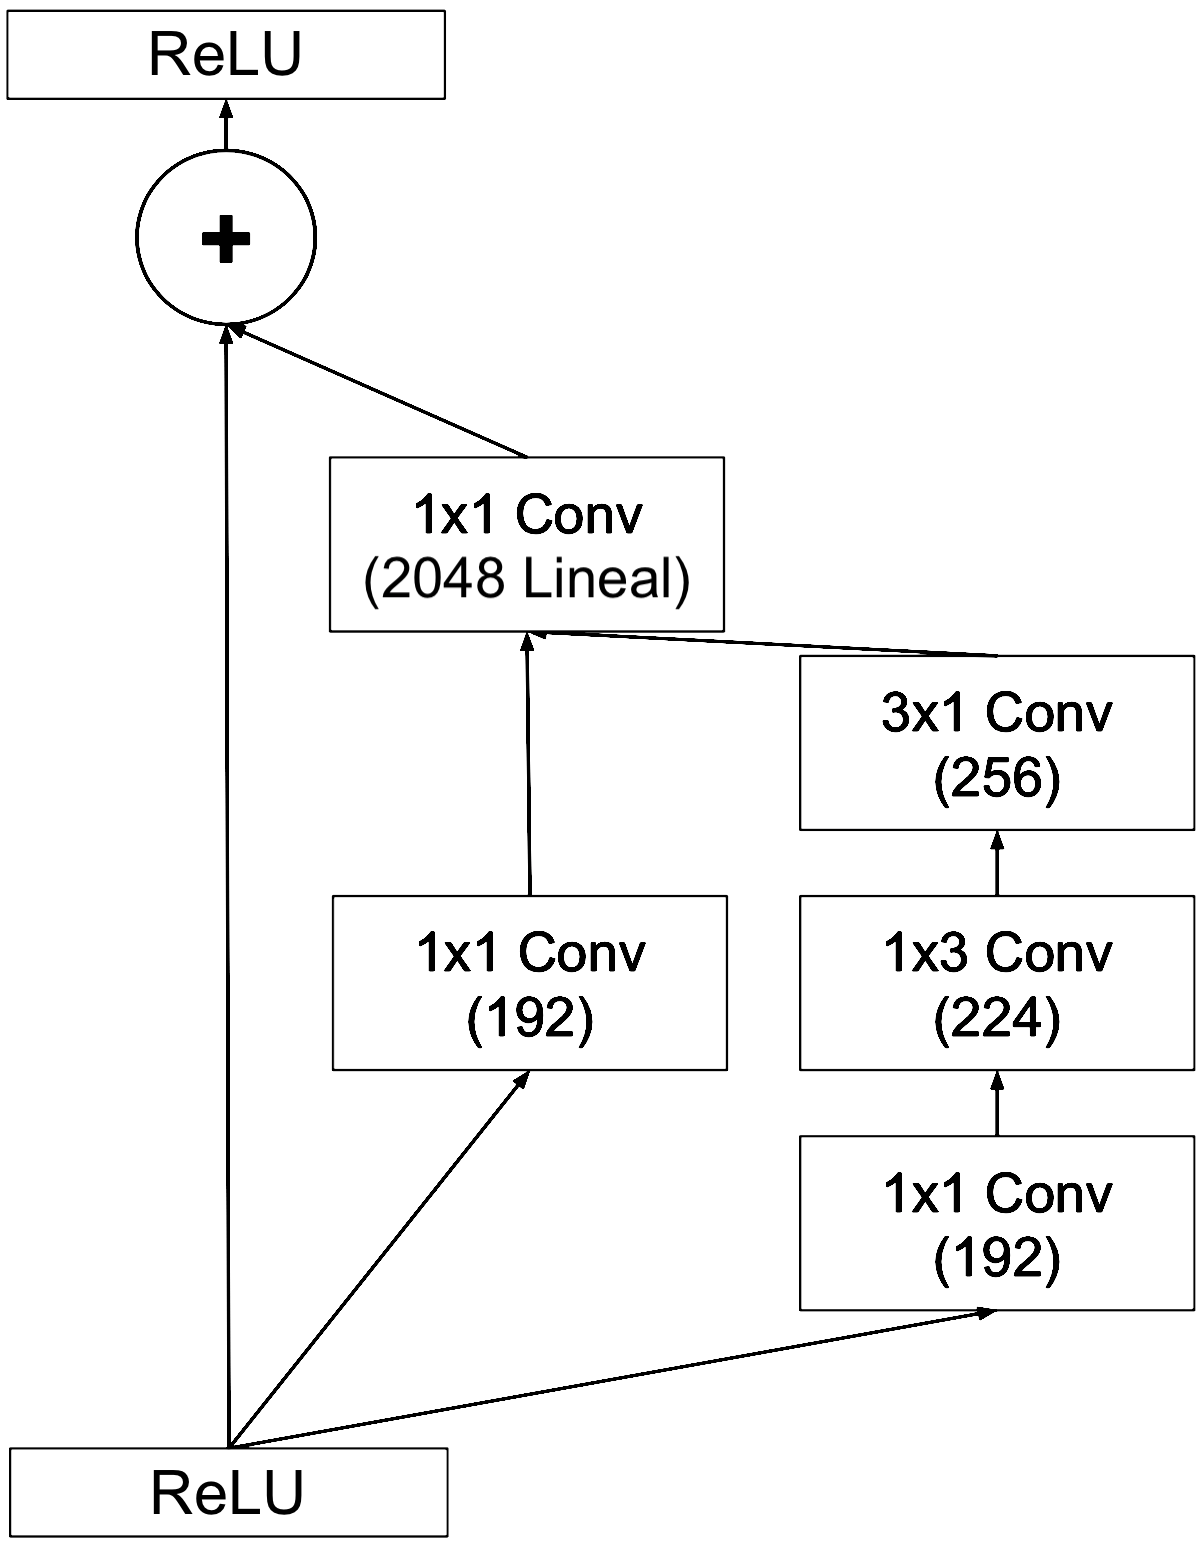
\includegraphics[width=.7\linewidth]{Images/Inception-ResNet-C.png}
      \caption{Bloque Inception-ResNet-C.}
      \label{fig:Inception-ResNet-C}
    \end{subfigure}
    
    \vspace{1cm}
    \begin{subfigure}[t]{.45\textwidth}
      \centering
      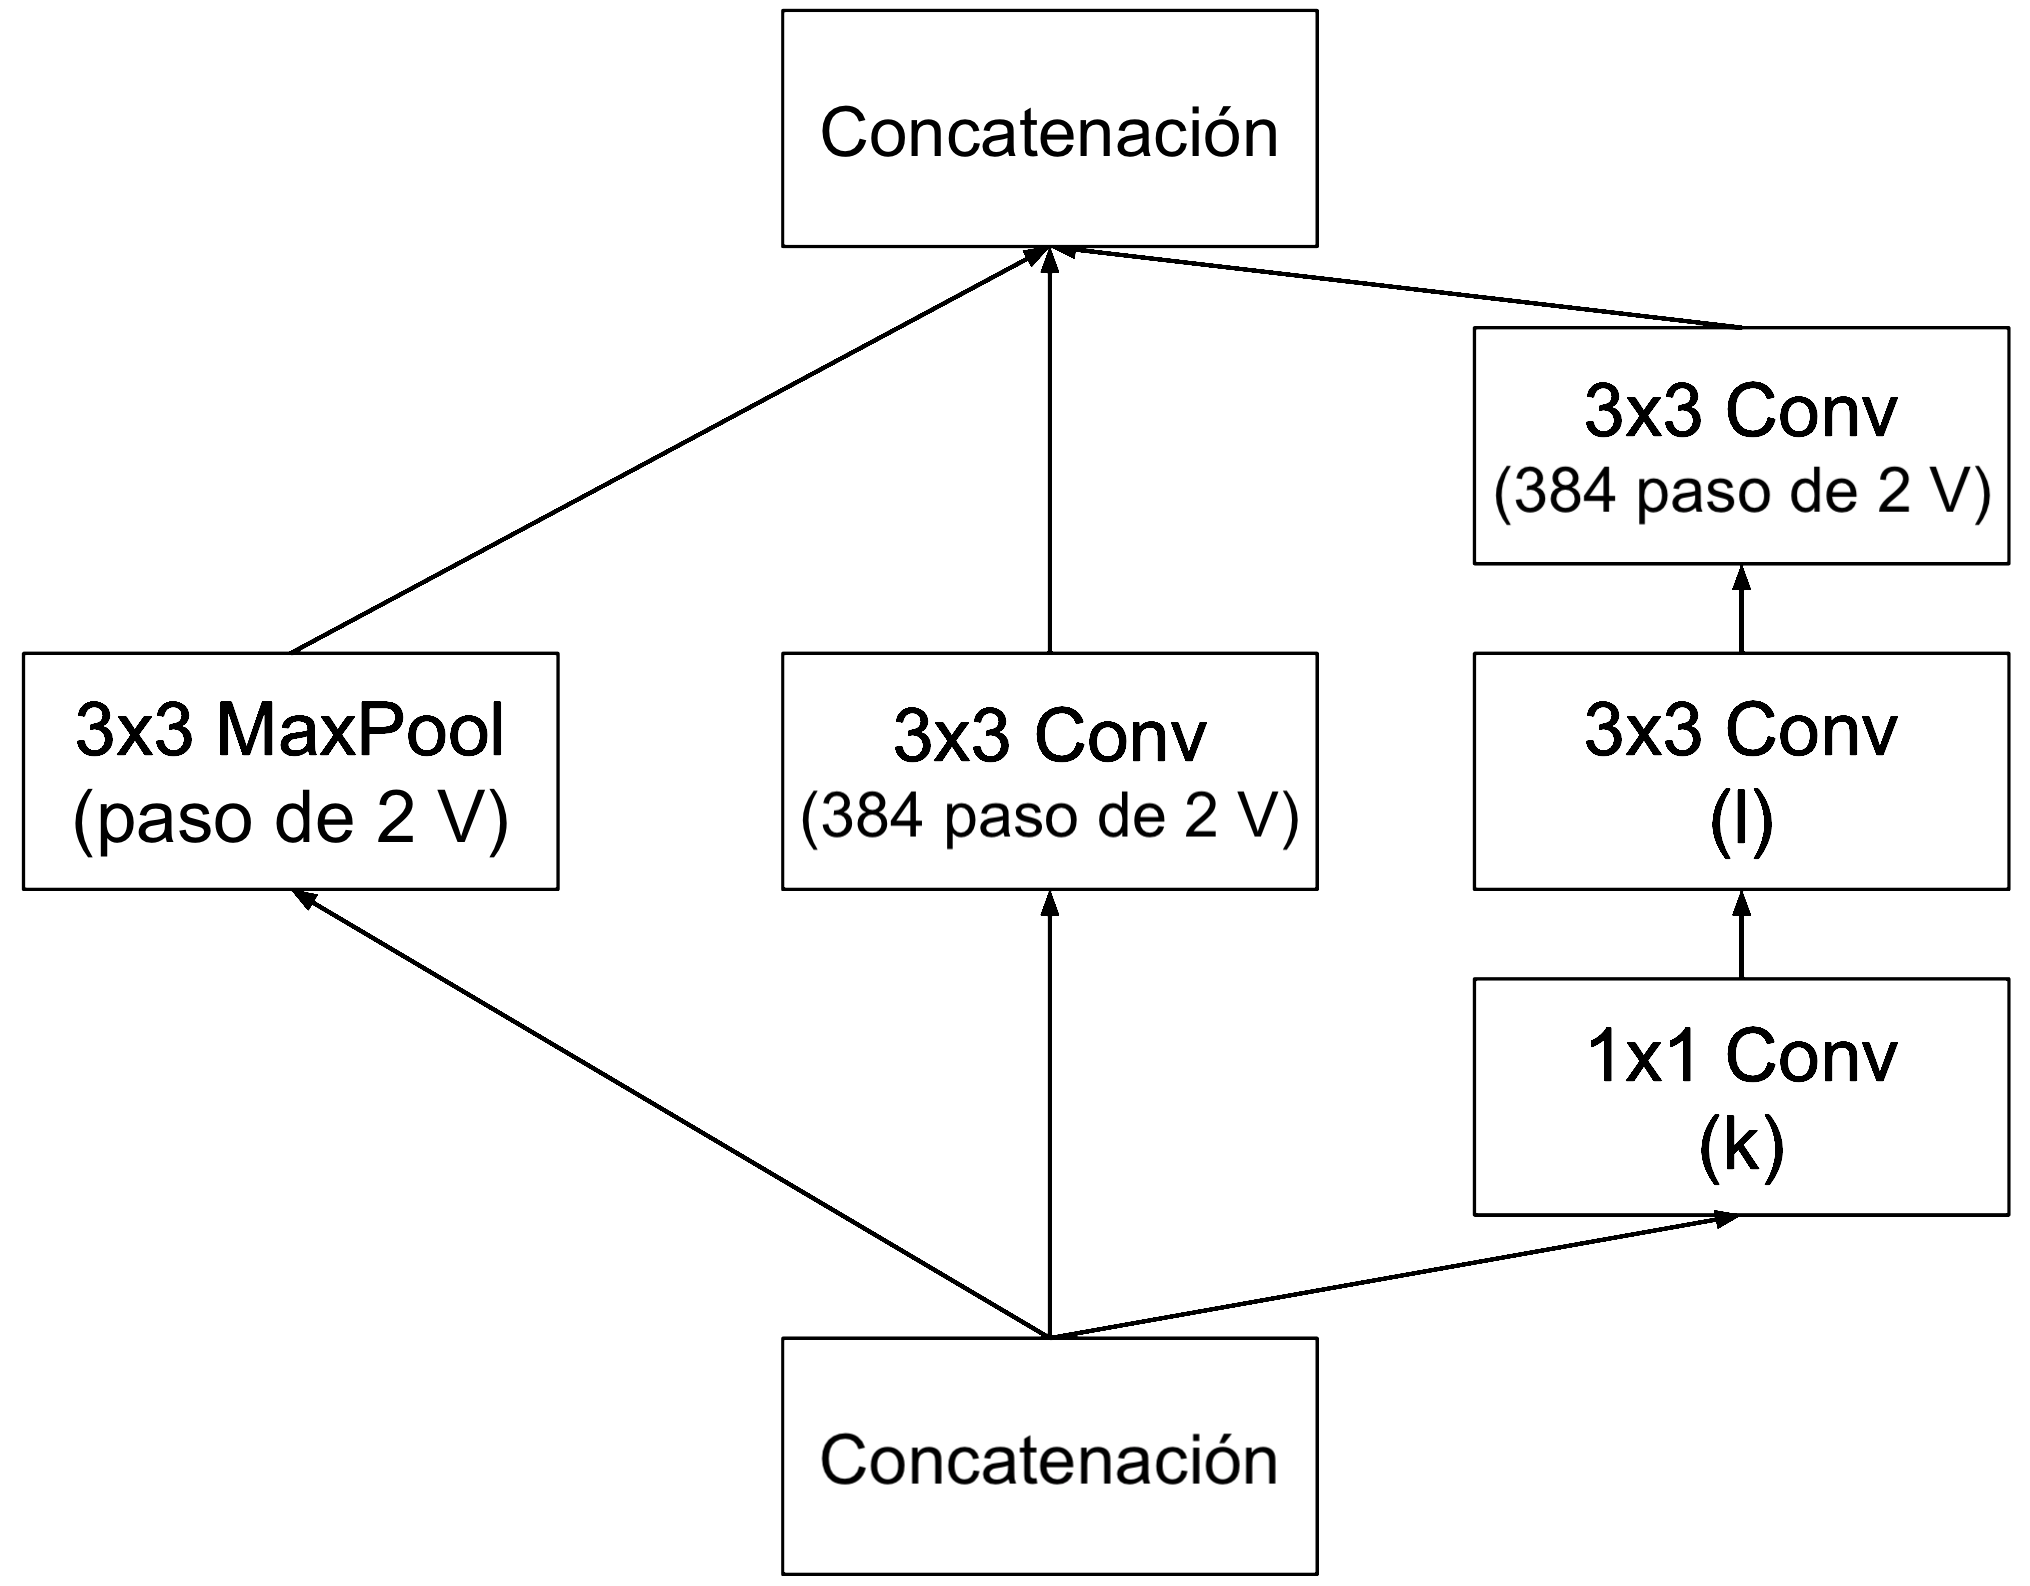
\includegraphics[width=.9\linewidth]{Images/Reduction-A.png}
      \caption{Bloque Reduction-A.}
      \label{fig:Reduction-A}
    \end{subfigure}
    \hfill
    \begin{subfigure}[t]{.45\textwidth}
      \centering
      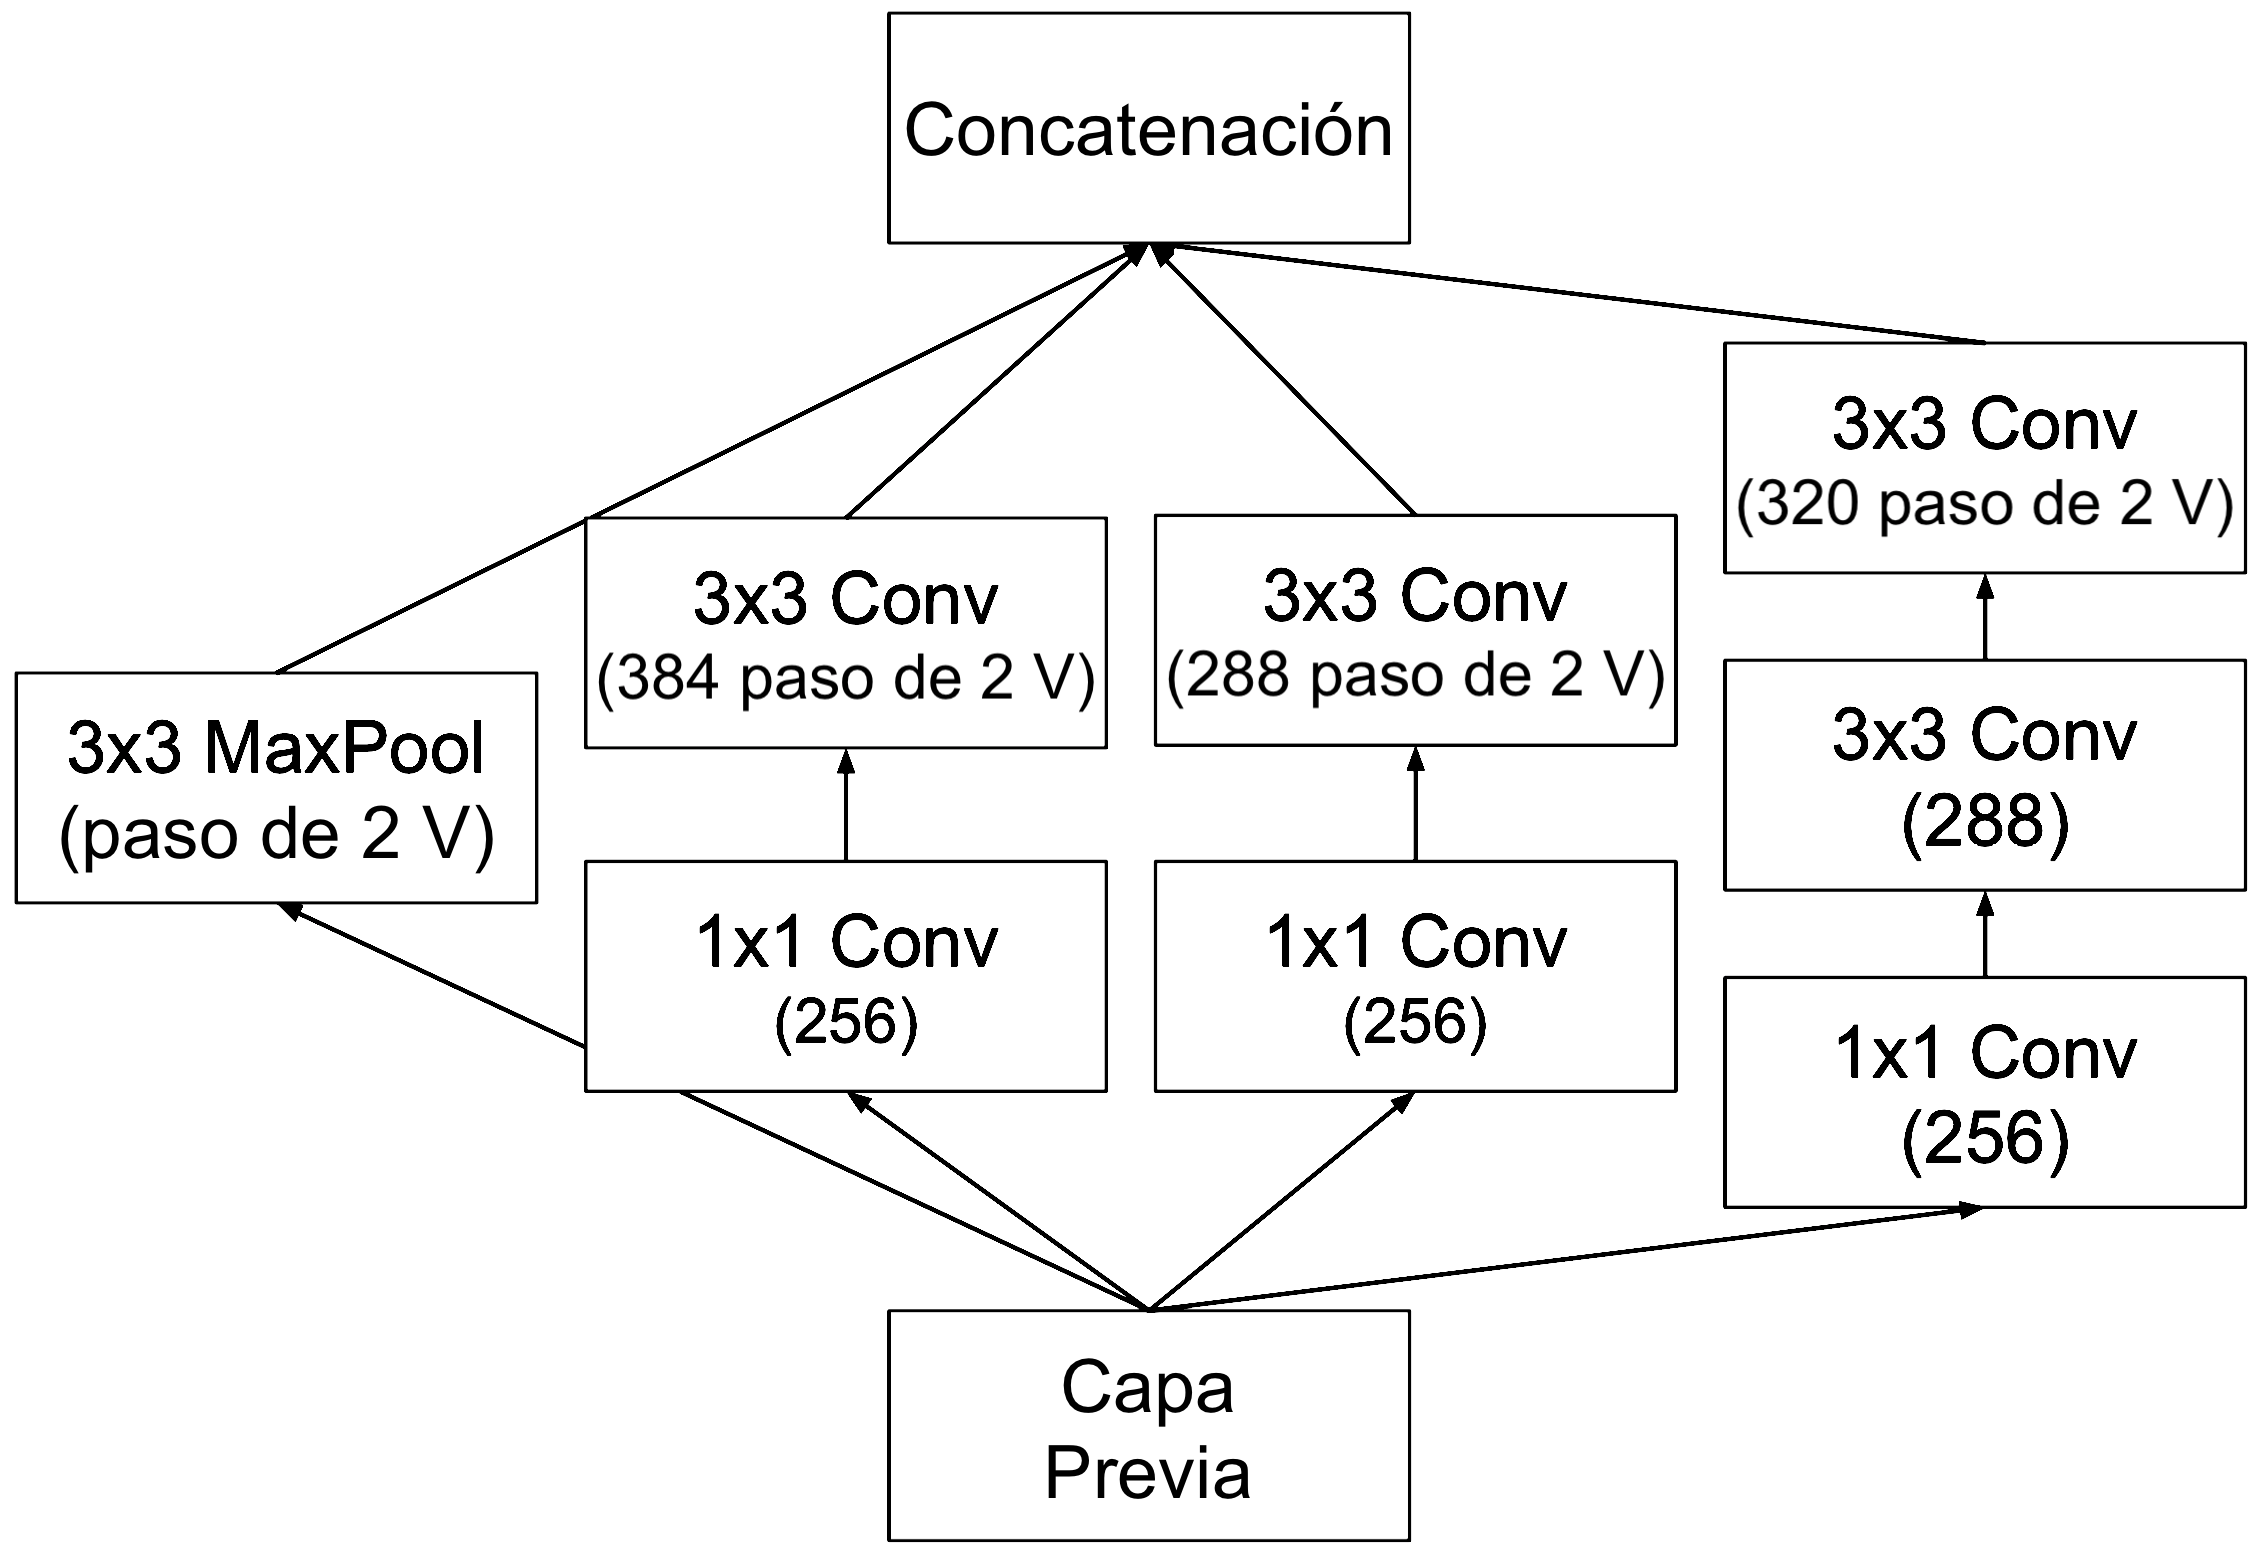
\includegraphics[width=.9\linewidth]{Images/Reduction-B.png}
      \caption{Bloque Reduction-B.}
      \label{fig:Reduction-B}
    \end{subfigure}
    \caption{Módulos empleados en la arquitectura Inception-ResNet-v2 \cite{Inception-ResNet}.}
    \label{fig:Inception-ResNet-v2Modules}
\end{figure}

%% INCEPTION-V3

\begin{figure}
   \vspace{1cm}
    \begin{subfigure}[t]{\textwidth}
      \centering
      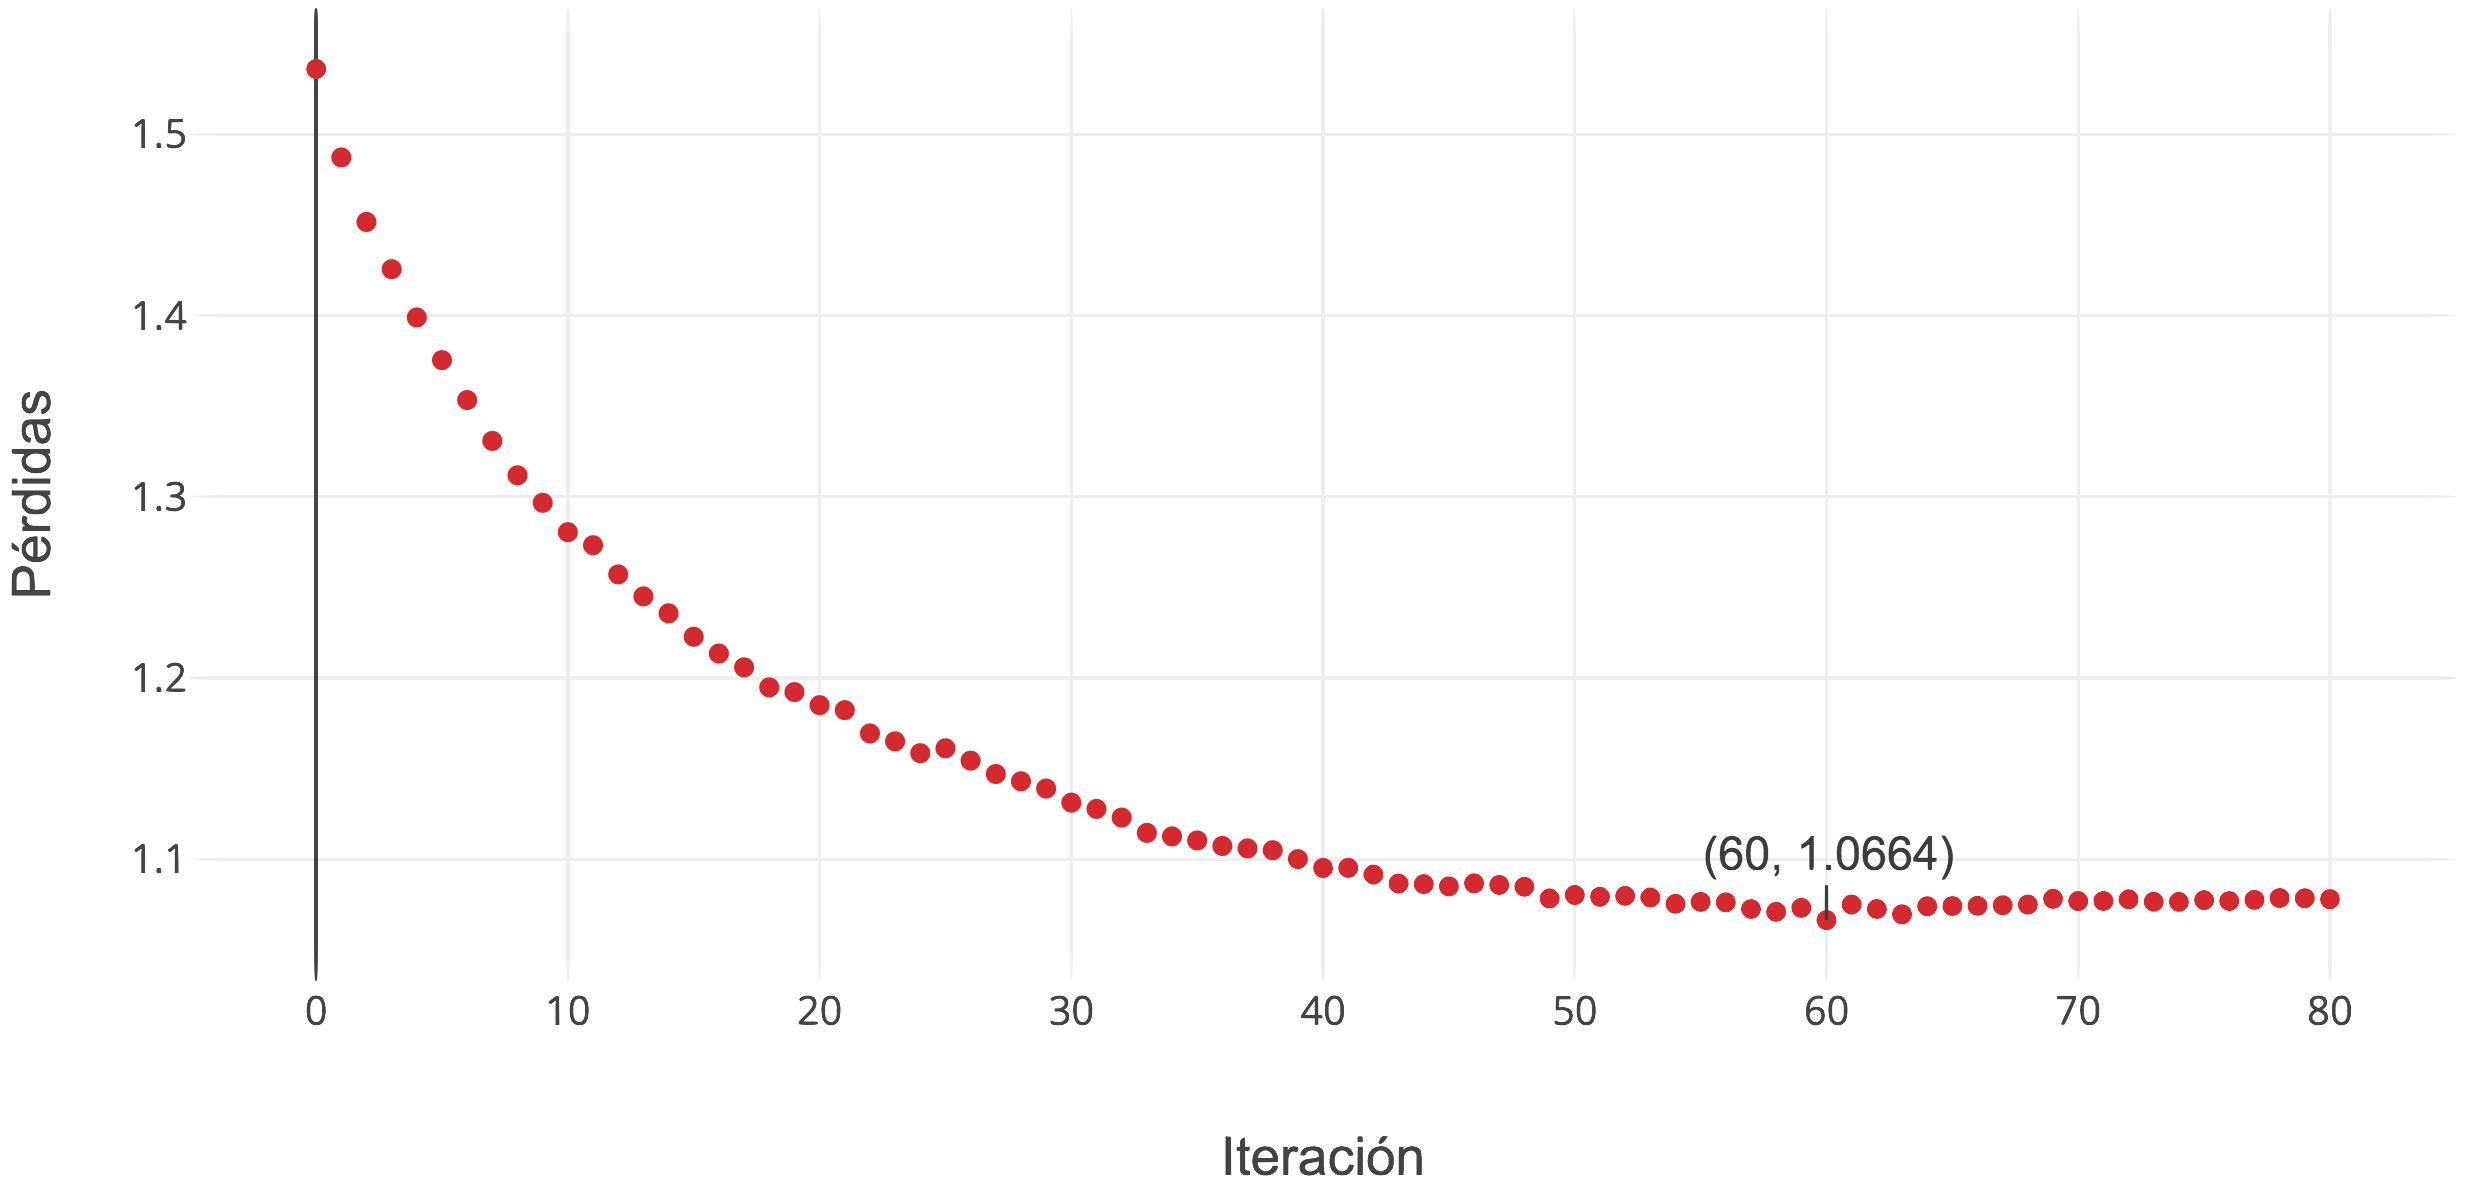
\includegraphics[width=\linewidth]{Images/Inception-v3_loss.png}
      \caption{Pérdidas calculadas a lo largo del entrenamiento del modelo Inception-v3.}
      \label{fig:Inception-v3_loss}
    \end{subfigure}
    
    \vspace{1cm}
    \begin{subfigure}[t]{\textwidth}
      \centering
      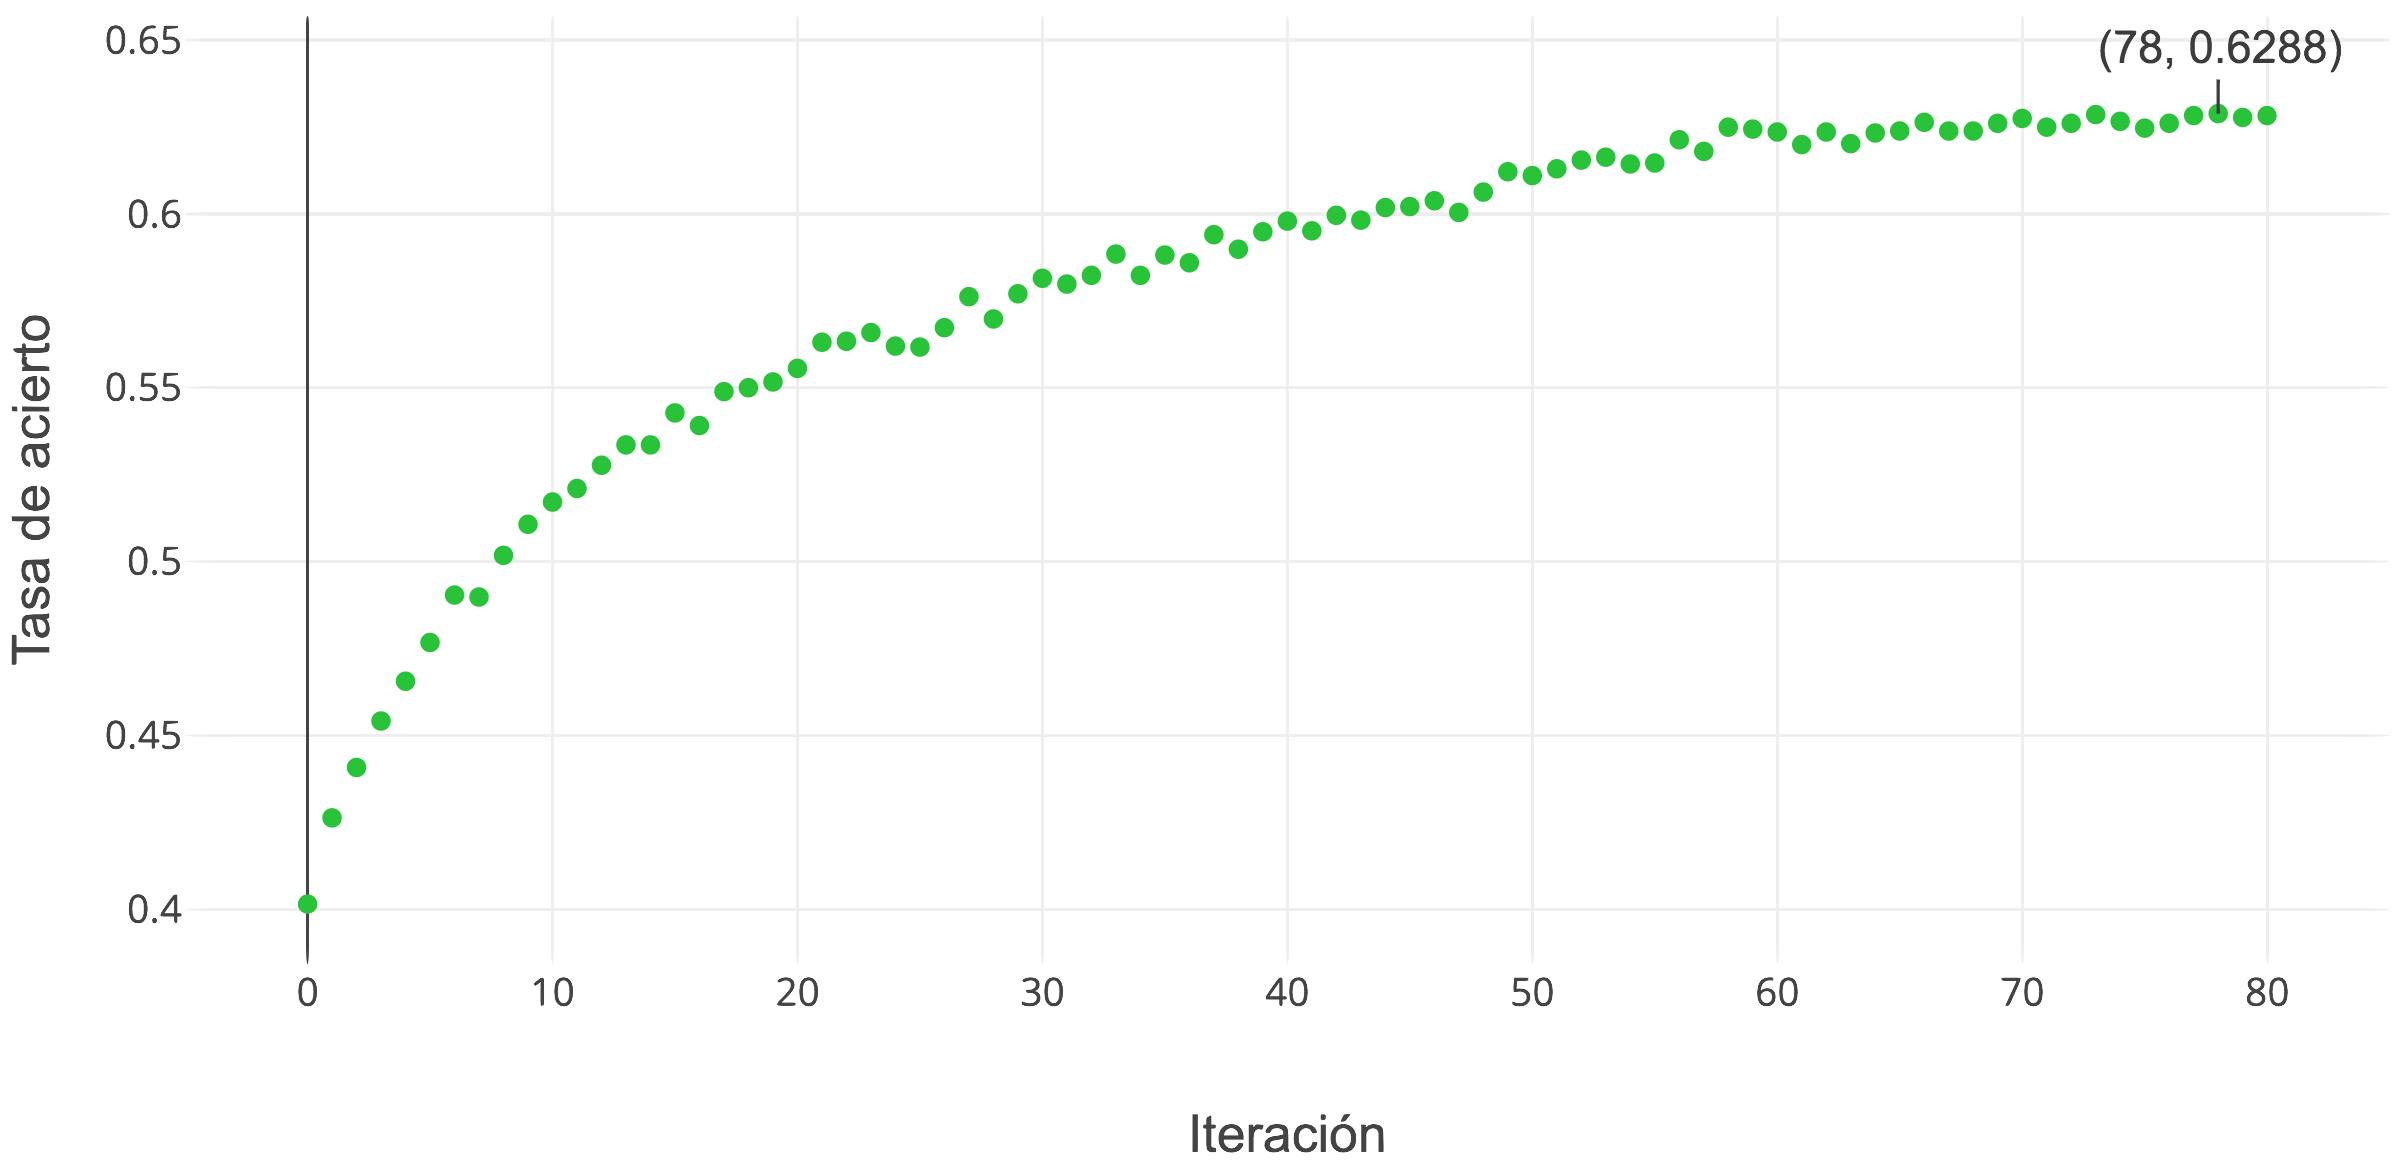
\includegraphics[width=\linewidth]{Images/Inception-v3_acc.png}
      \caption{Tasas de acierto calculadas a lo largo del entrenamiento del modelo Inception-v3.}
      \label{fig:Inception-v3_acc}
    \end{subfigure}
    \caption{Métricas calculadas a lo largo del entrenamiento del modelo Inception-v3 sobre el conjunto de validación de la base de datos FER-2013.}
    \label{fig:Inception-v3_metrics}
\end{figure}

\begin{figure}
    \centering
    \begin{subfigure}[t]{\textwidth}
      \centering
      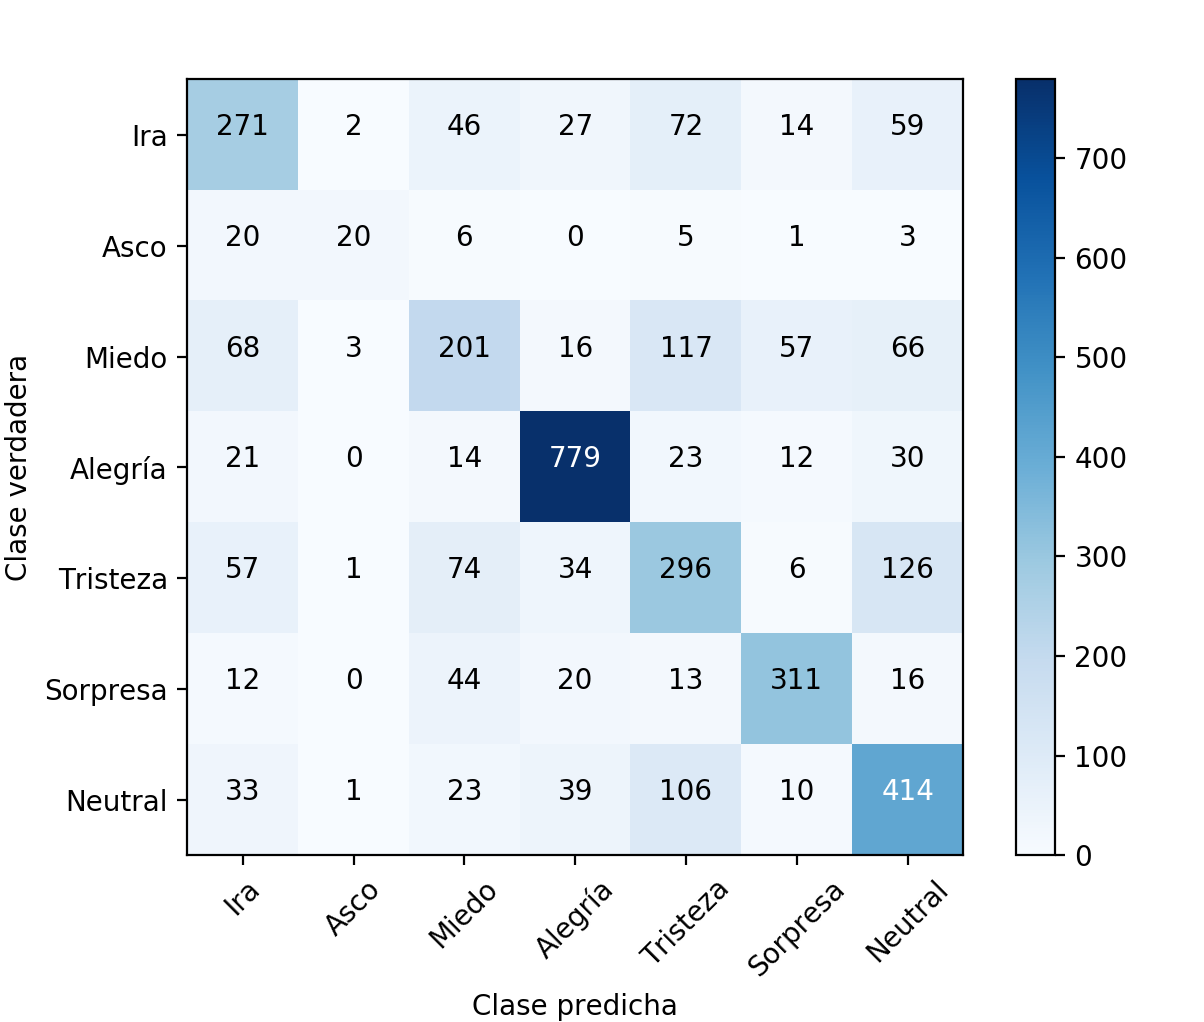
\includegraphics[width=0.7\linewidth]{Images/Inception-v3_matrix.png}
      \caption{Matriz de confusión del modelo Inception-v3.}
      \label{fig:Inception-v3_matrix}
    \end{subfigure}
    
    \vspace{1cm}
    \begin{subfigure}[t]{\textwidth}
      \centering
      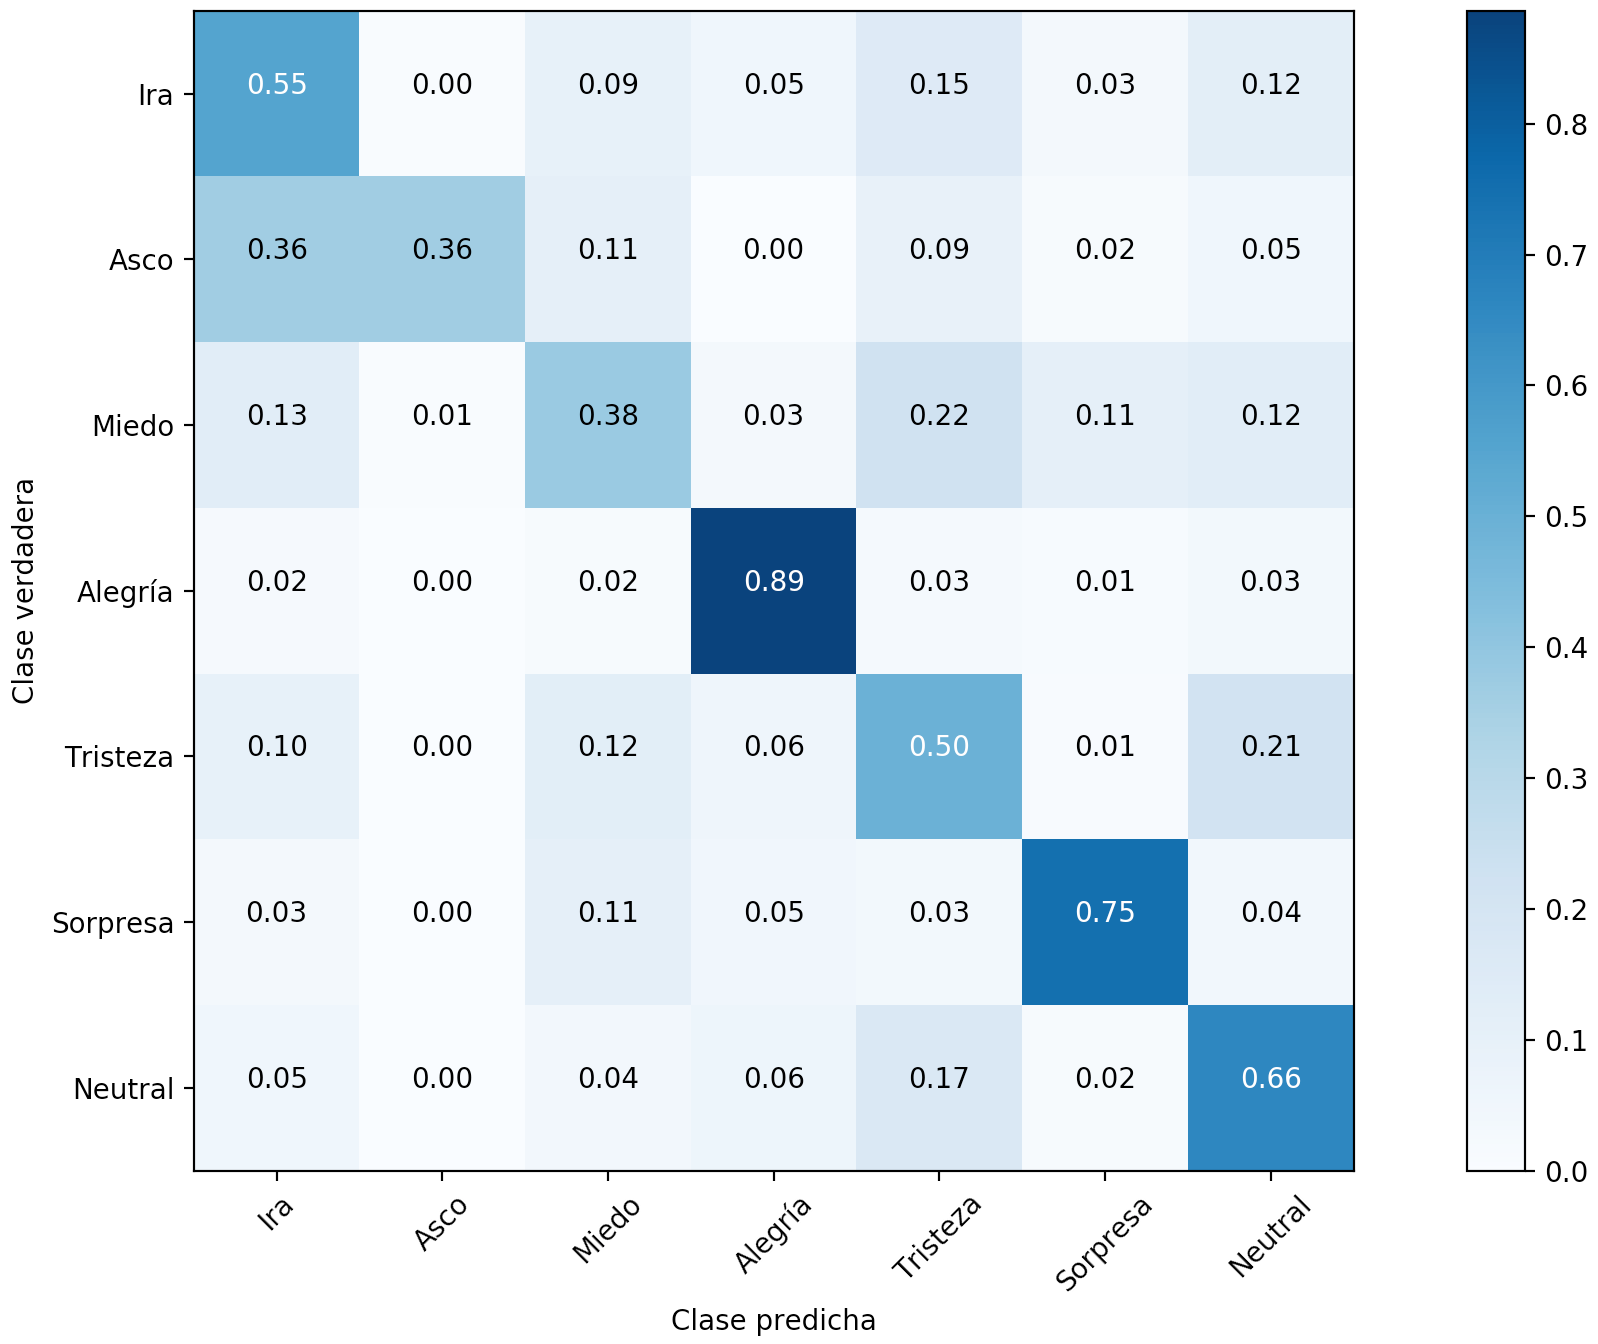
\includegraphics[width=0.7\linewidth]{Images/Inception-v3_matrix_norm.png}
      \caption{Matriz de confusión normalizada del modelo Inception-v3.}
      \label{fig:Inception-v3_matrix_norm}
    \end{subfigure}
    \caption{Matrices de confusión del conjunto de evaluación de la base de datos FER-2013 estimadas sobre el modelo entrenado Inception-v3.}
    \label{fig:Inception-v3_matrices}
\end{figure}

%% INCEPTION-RESNET-V2

\begin{figure}
   \vspace{1cm}
    \begin{subfigure}[t]{\textwidth}
      \centering
      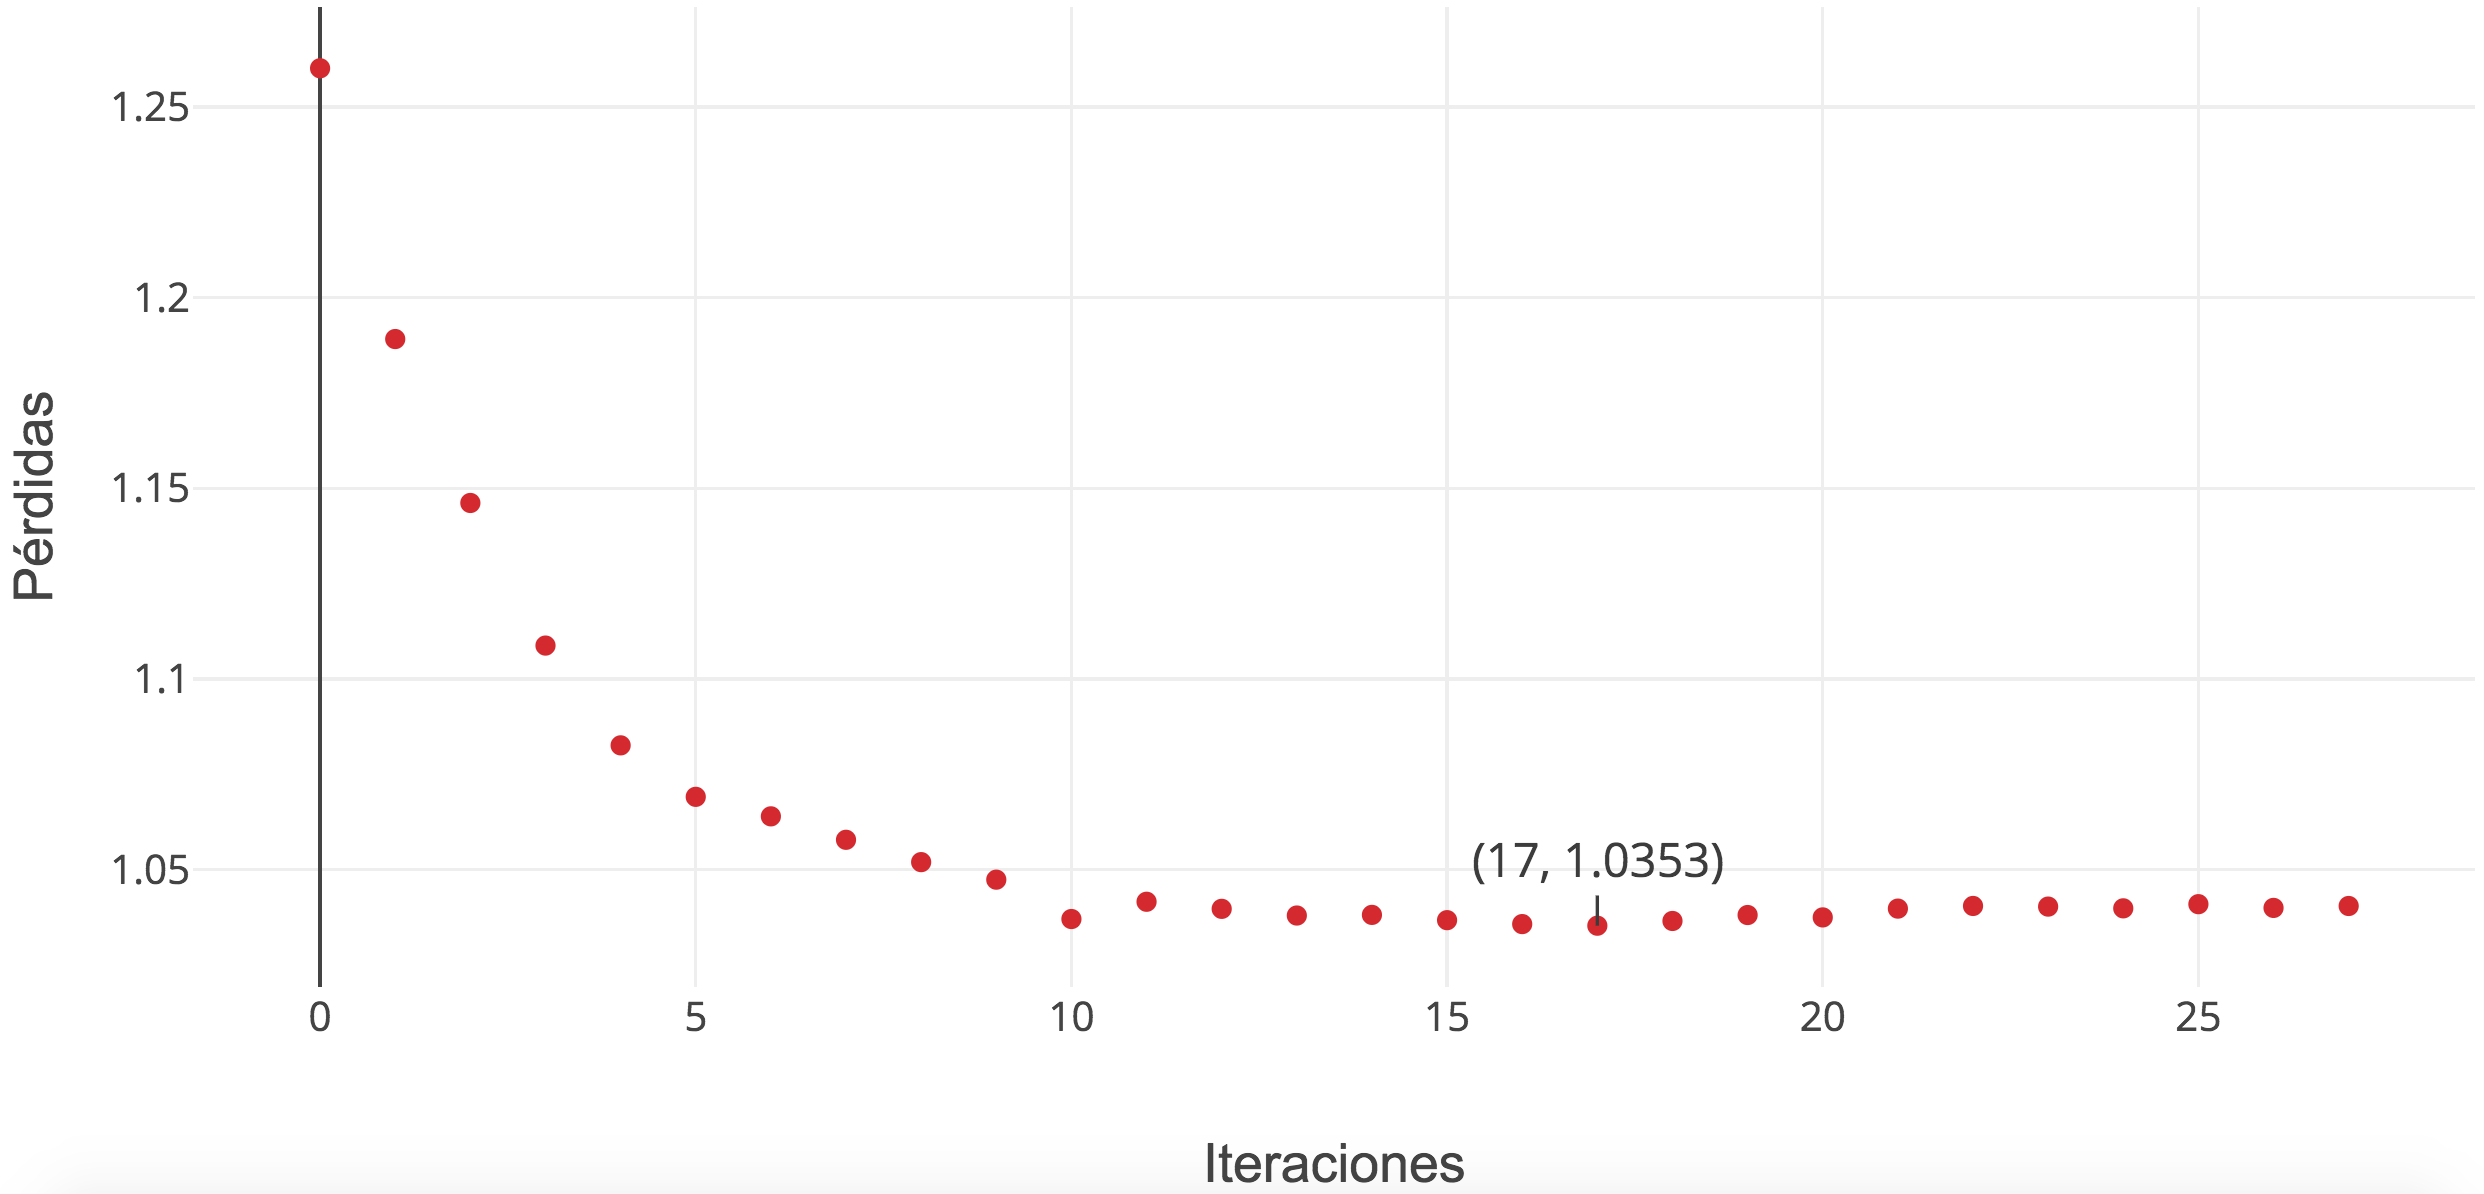
\includegraphics[width=\linewidth]{Images/Inception-ResNet-v2_loss.png}
      \caption{Pérdidas calculadas a lo largo del entrenamiento del modelo Inception-ResNet-v2.}
      \label{fig:Inception-ResNet-v2_loss}
    \end{subfigure}
    
    \vspace{1cm}
    \begin{subfigure}[t]{\textwidth}
      \centering
      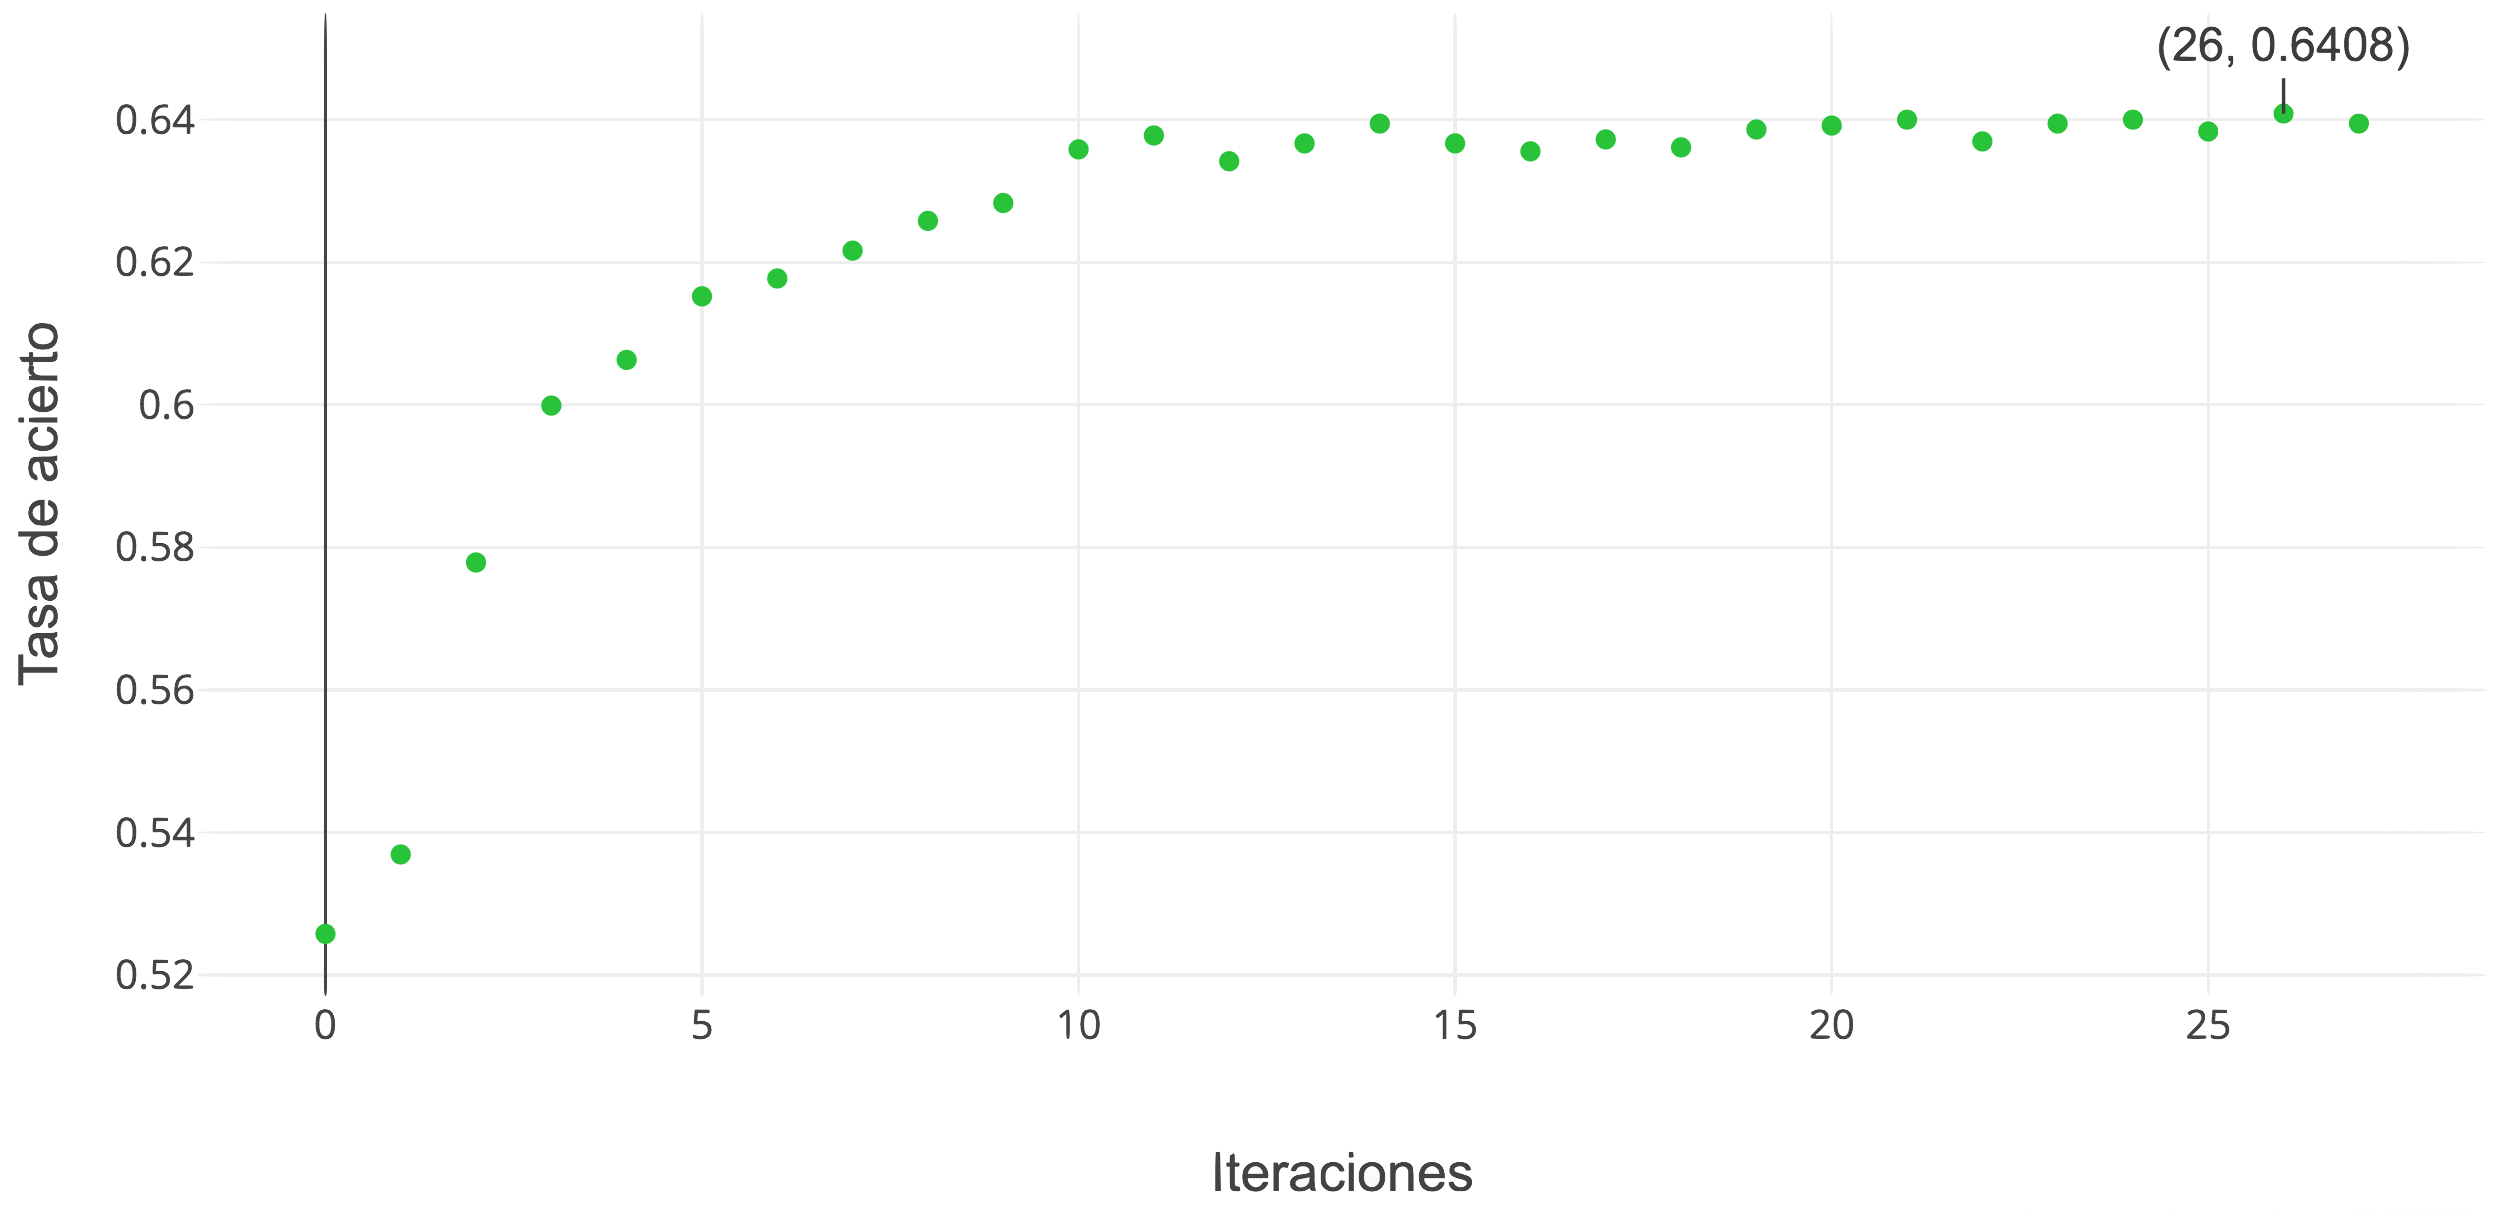
\includegraphics[width=\linewidth]{Images/Inception-ResNet-v2_acc.png}
      \caption{Tasas de acierto calculadas a lo largo del entrenamiento del modelo Inception-ResNet-v2.}
      \label{fig:Inception-ResNet-v2_acc}
    \end{subfigure}
    \caption{Métricas calculadas a lo largo del entrenamiento del modelo Inception-ResNet-v2 sobre el conjunto de validación de la base de datos FER-2013.}
    \label{fig:Inception-ResNet-v2_metrics}
\end{figure}

\begin{figure}
    \centering
    \begin{subfigure}[t]{\textwidth}
      \centering
      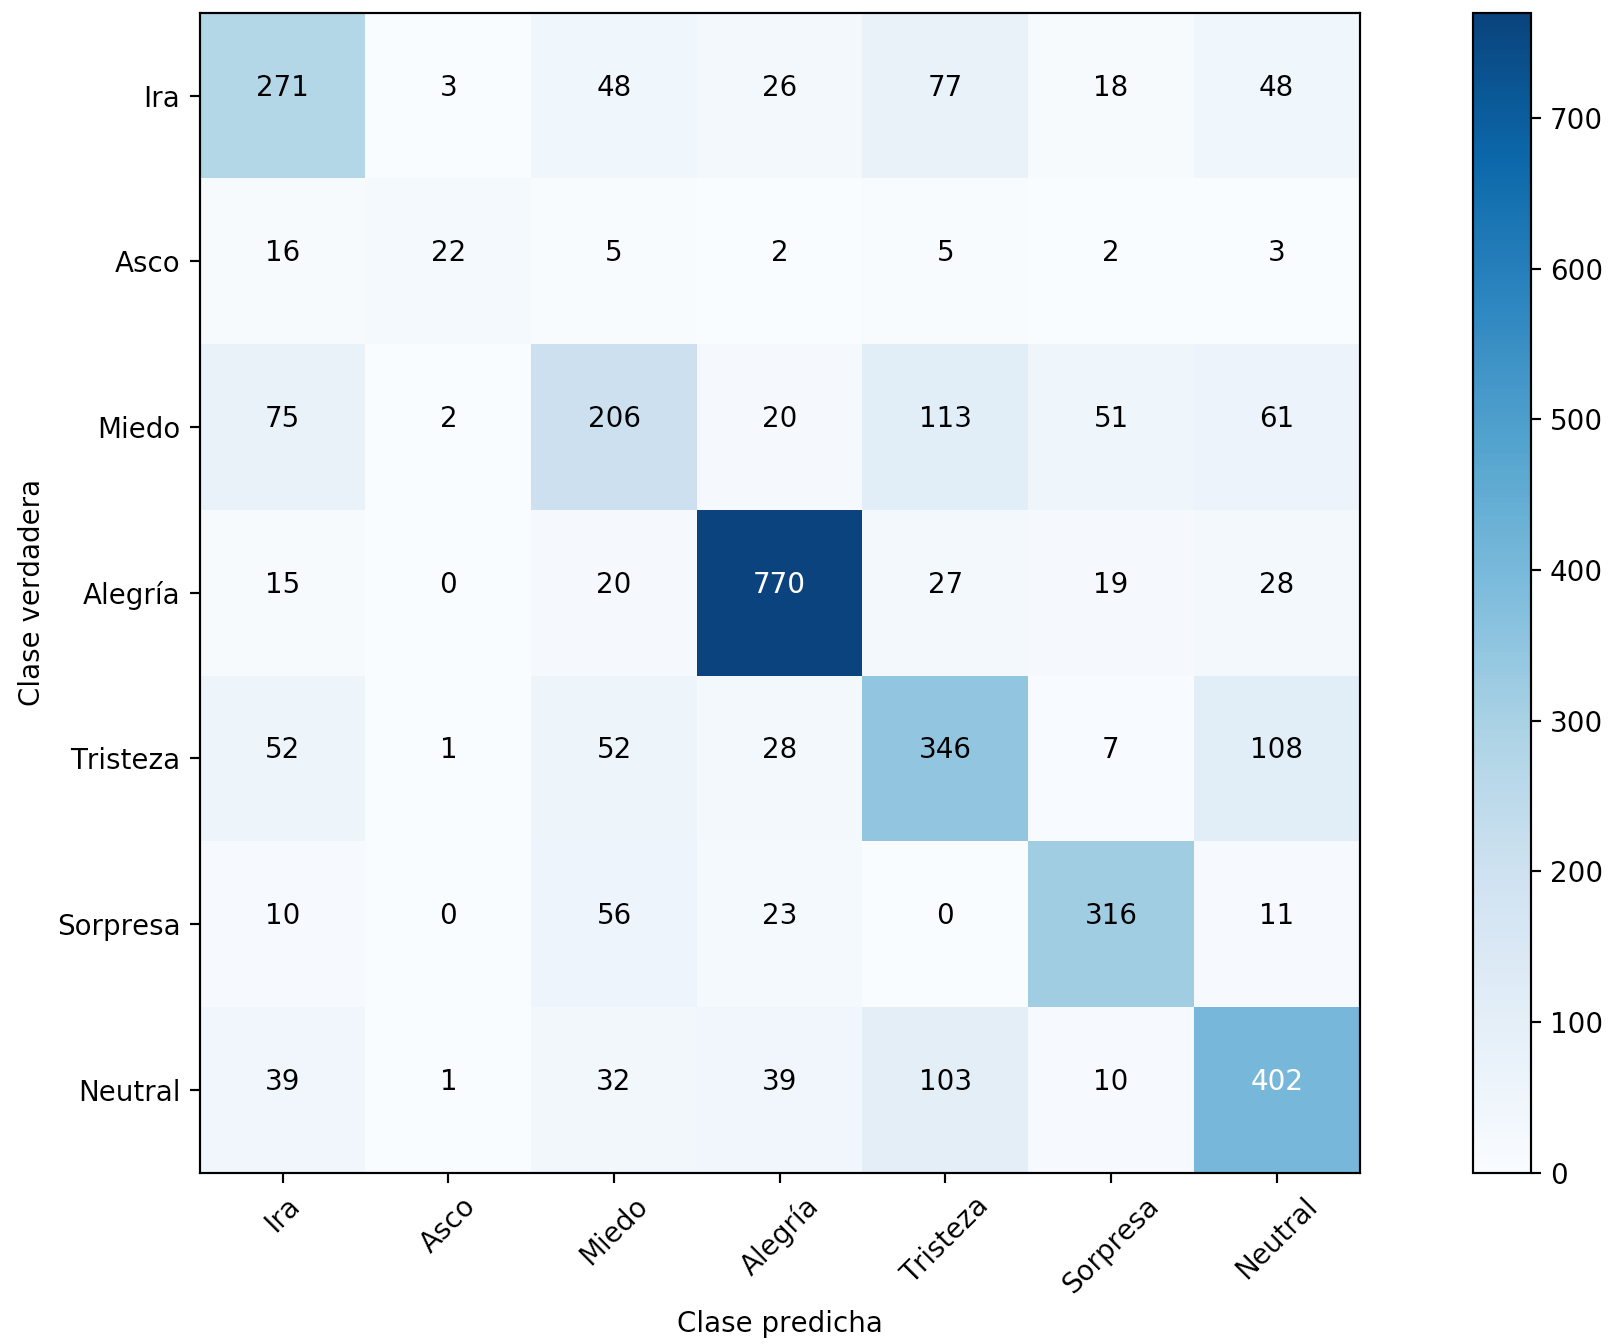
\includegraphics[width=0.7\linewidth]{Images/Inception-ResNet-v2_matrix.png}
      \caption{Matriz de confusión del modelo Inception-ResNet-v2.}
      \label{fig:Inception-ResNet-v2_matrix}
    \end{subfigure}
    
    \vspace{1cm}
    \begin{subfigure}[t]{\textwidth}
      \centering
      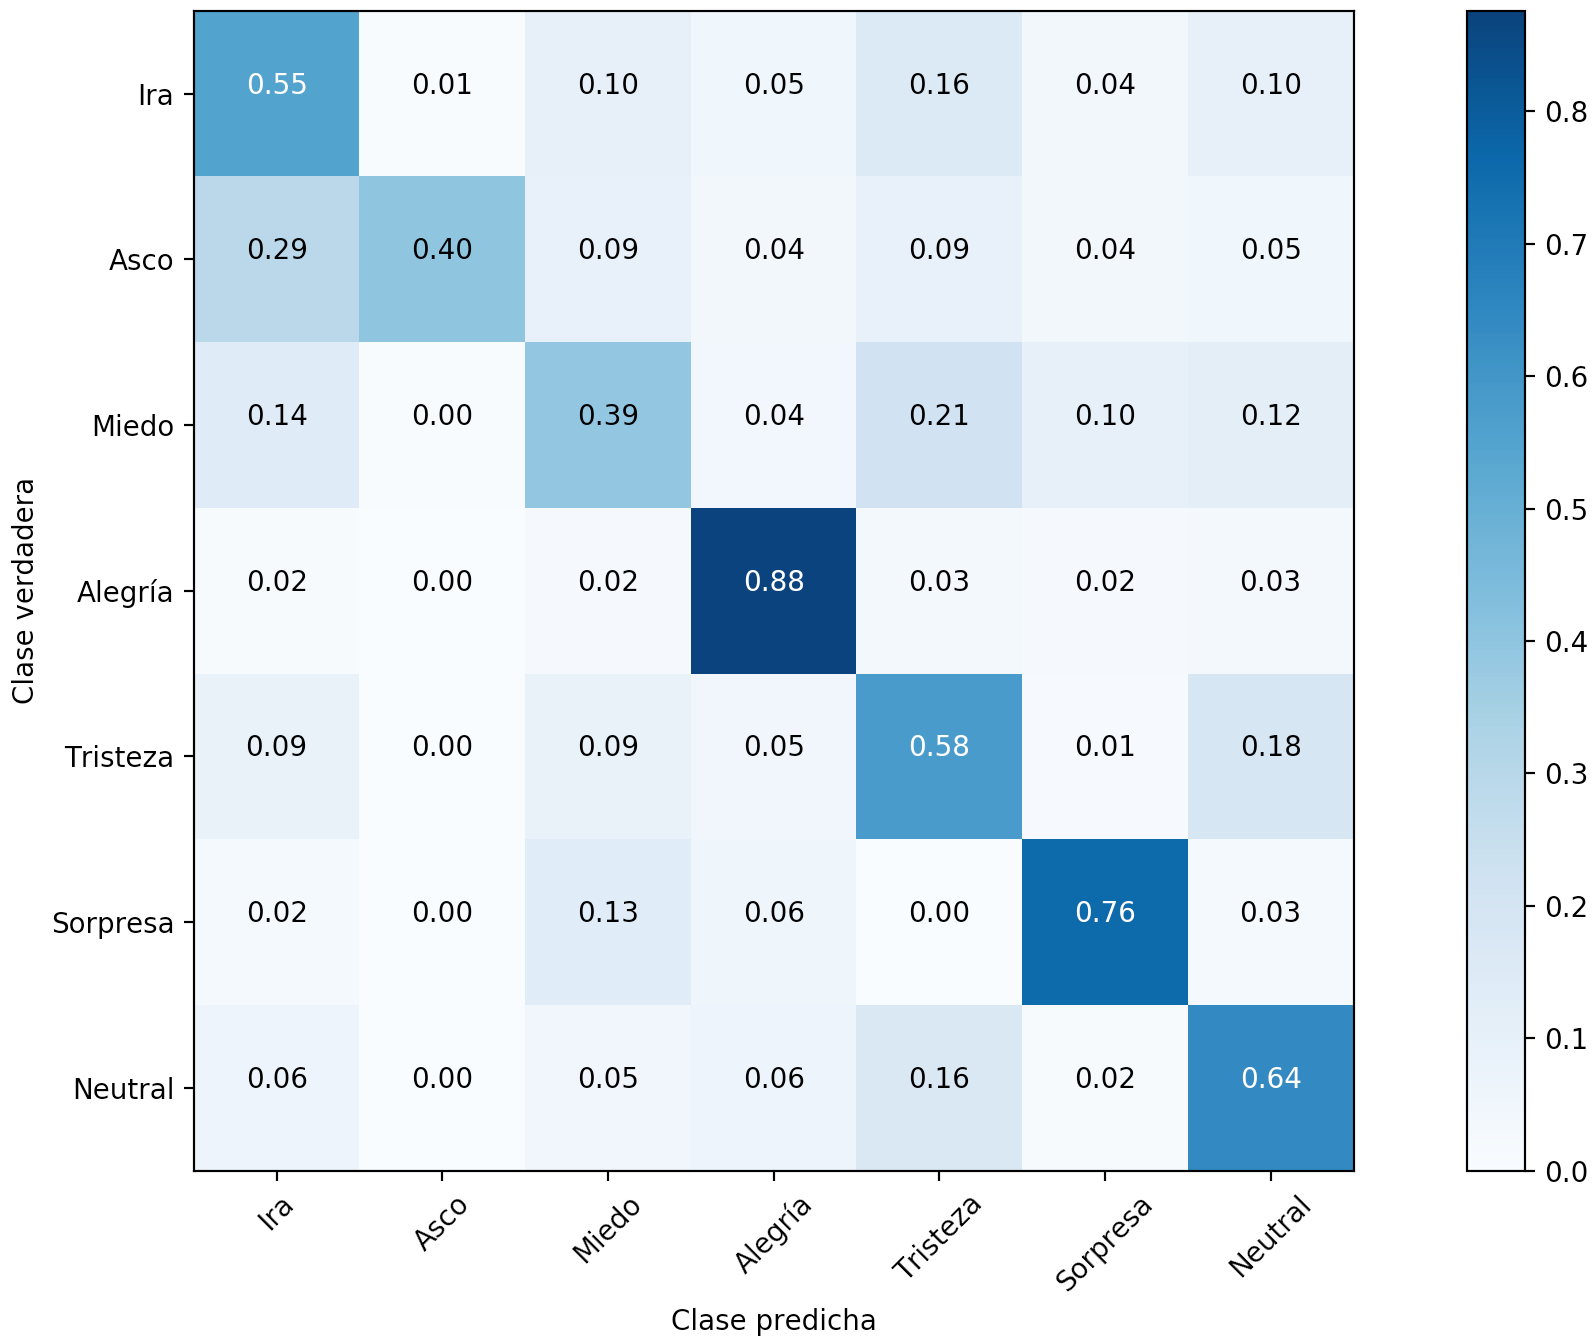
\includegraphics[width=0.7\linewidth]{Images/Inception-ResNet-v2_matrix_norm.png}
      \caption{Matriz de confusión normalizada del modelo Inception-ResNet-v2.}
      \label{fig:Inception-ResNet-v2_matrix_norm}
    \end{subfigure}
    \caption{Matrices de confusión del conjunto de evaluación de la base de datos FER-2013 estimadas sobre el modelo entrenado Inception-ResNet-v2.}
    \label{fig:Inception-ResNet-v2_matrices}
\end{figure}

%% RESNET-50

\begin{figure}
   \vspace{1cm}
    \begin{subfigure}[t]{\textwidth}
      \centering
      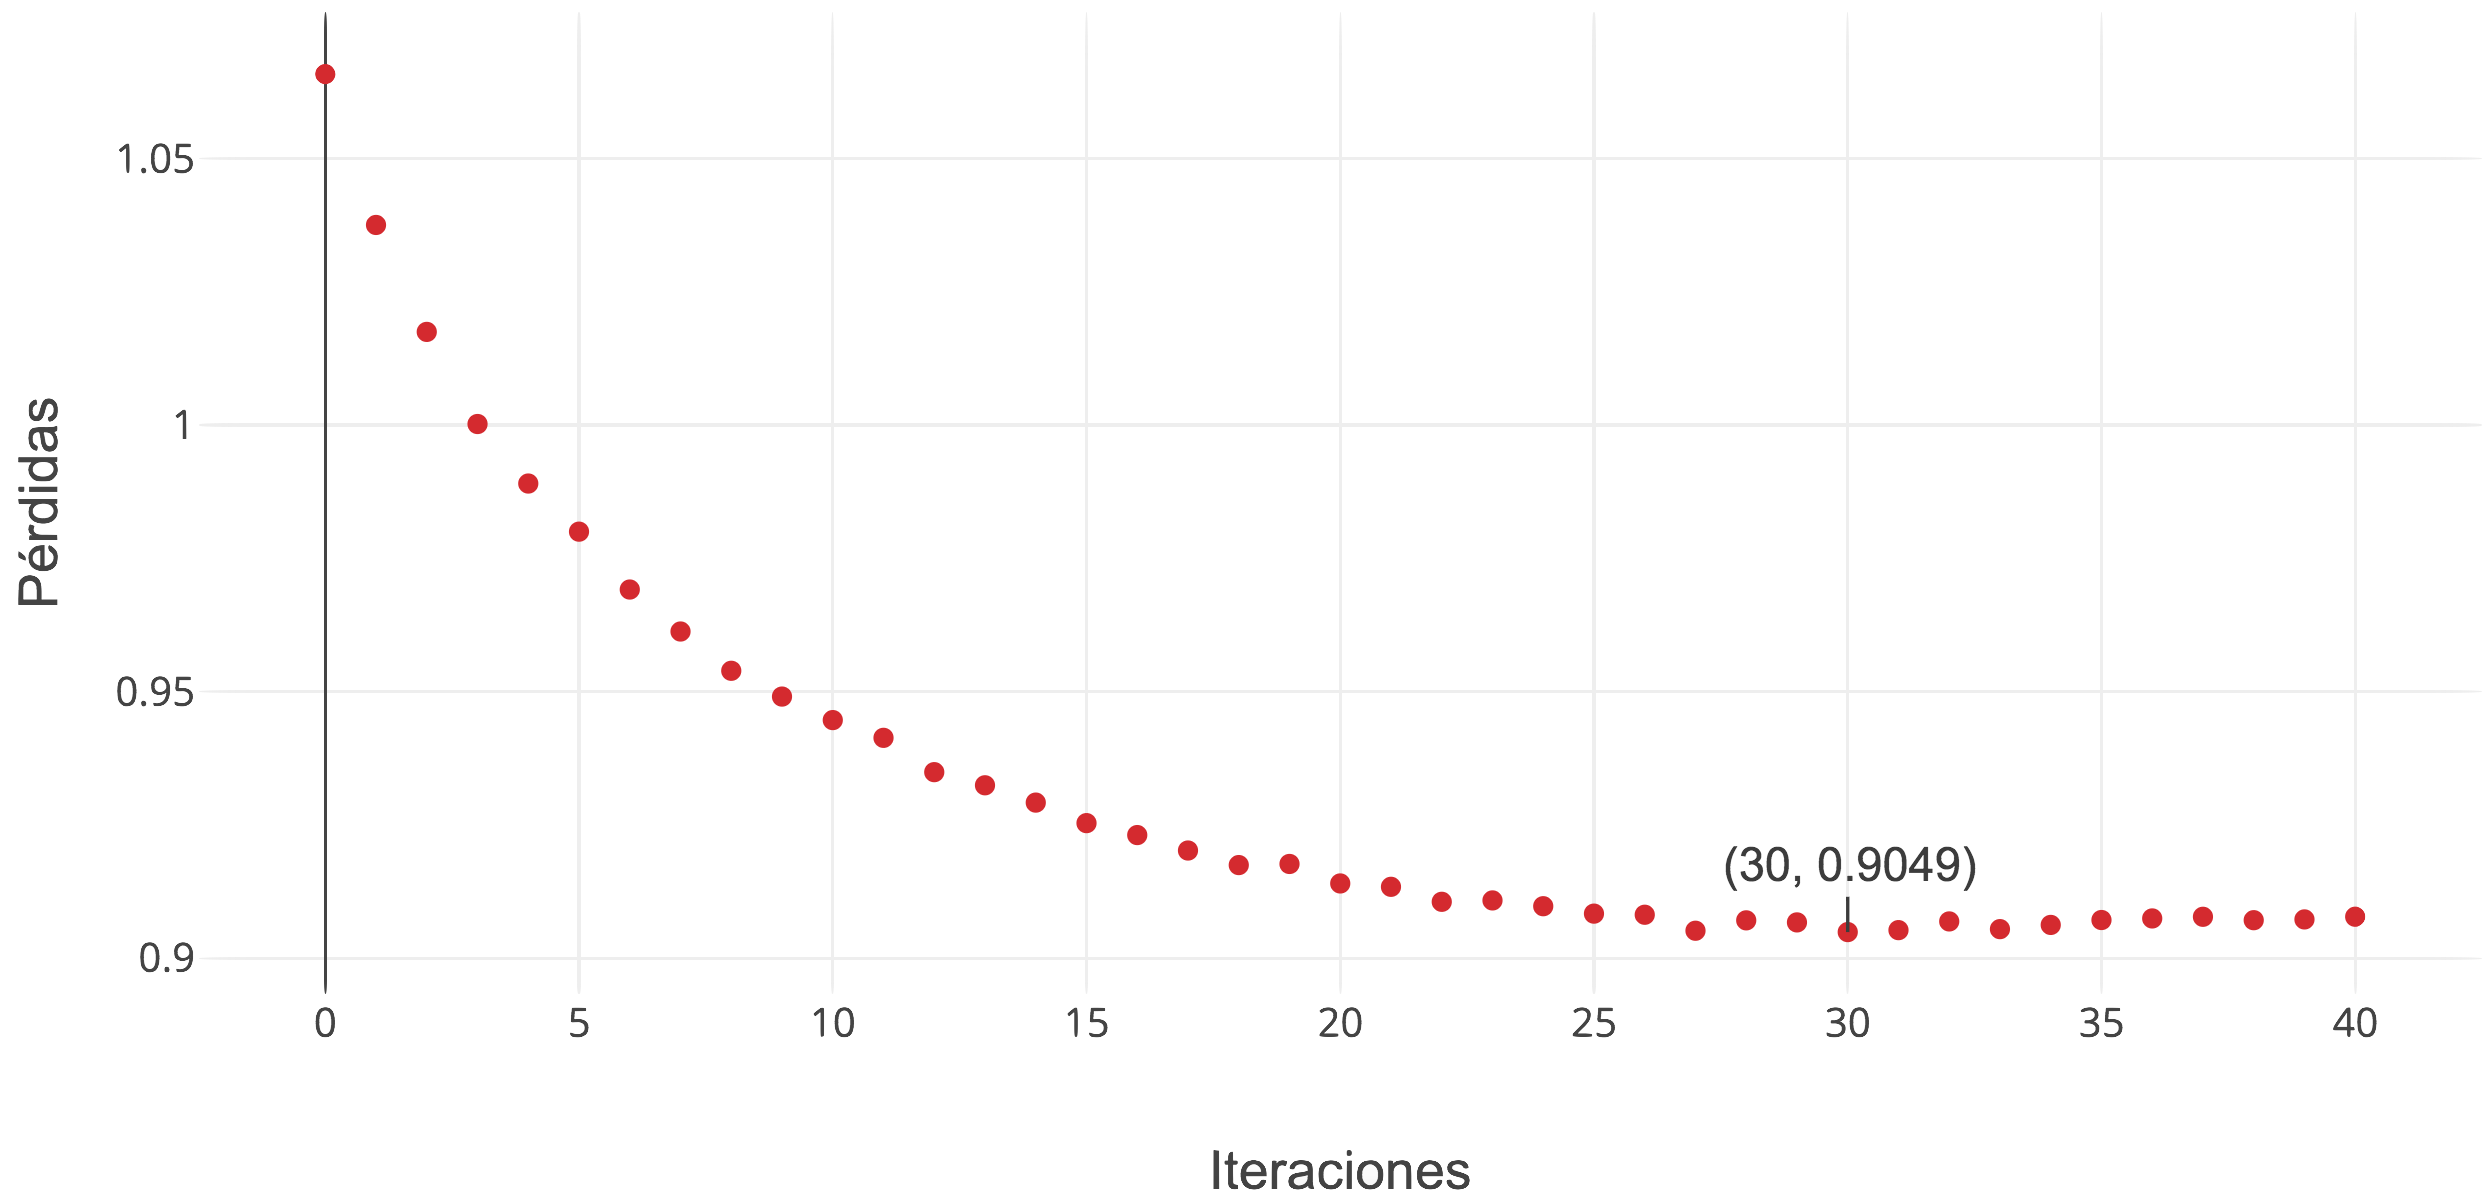
\includegraphics[width=\linewidth]{Images/ResNet-50_loss.png}
      \caption{Pérdidas calculadas a lo largo del entrenamiento del modelo ResNet-50.}
      \label{fig:ResNet-50_loss}
    \end{subfigure}
    
    \vspace{1cm}
    \begin{subfigure}[t]{\textwidth}
      \centering
      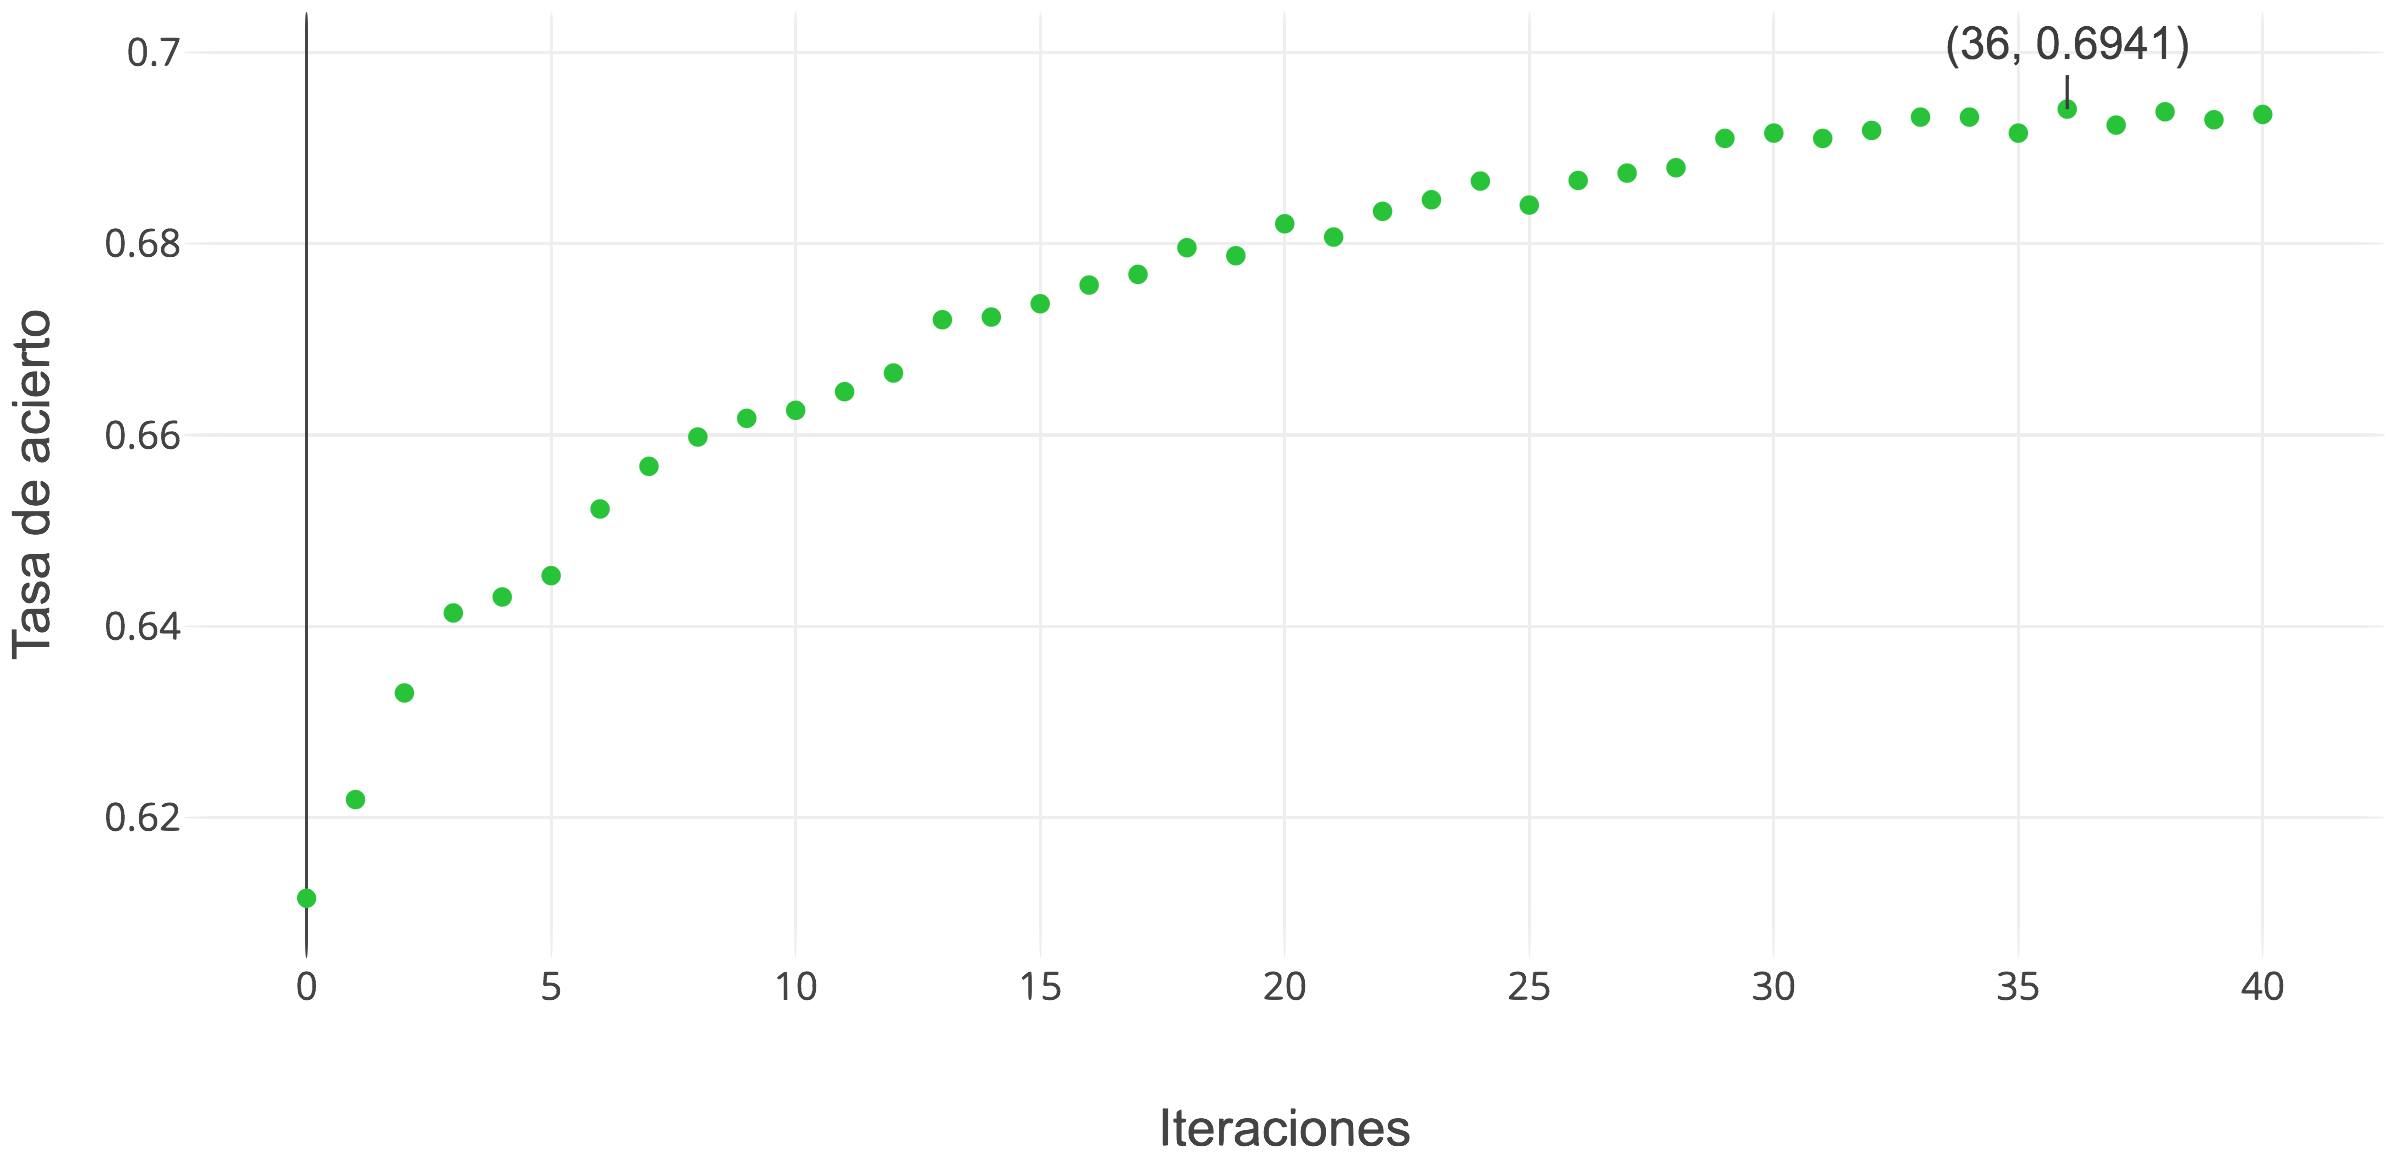
\includegraphics[width=\linewidth]{Images/ResNet-50_acc.png}
      \caption{Tasas de acierto calculadas a lo largo del entrenamiento del modelo ResNet-50.}
      \label{fig:ResNet-50_acc}
    \end{subfigure}
    \caption{Métricas calculadas a lo largo del entrenamiento del modelo ResNet-50 sobre el conjunto de validación de la base de datos FER-2013.}
    \label{fig:ResNet-50_metrics}
\end{figure}

\begin{figure}
    \centering
    \begin{subfigure}[t]{\textwidth}
      \centering
      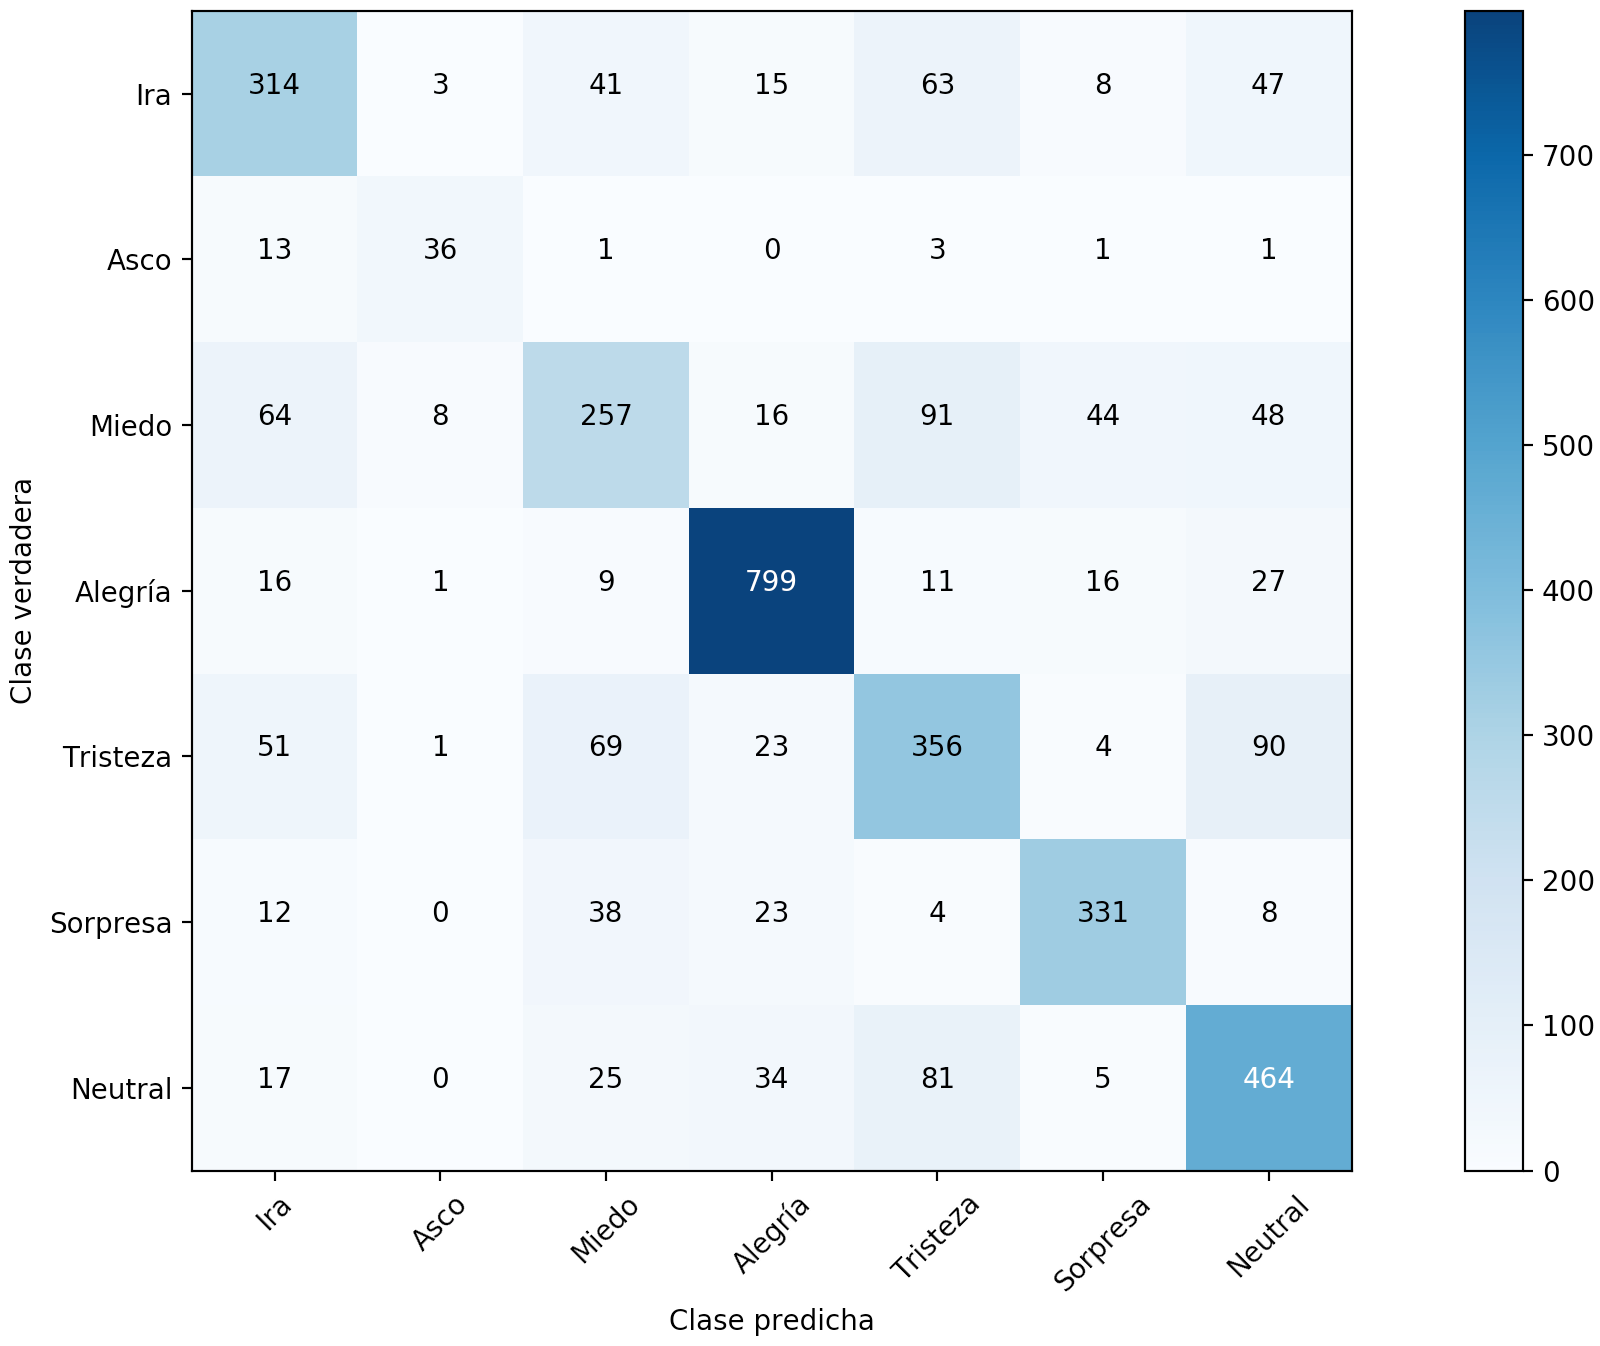
\includegraphics[width=0.7\linewidth]{Images/ResNet-50_matrix.png}
      \caption{Matriz de confusión del modelo ResNet-50.}
      \label{fig:ResNet-50_matrix}
    \end{subfigure}
    
    \vspace{1cm}
    \begin{subfigure}[t]{\textwidth}
      \centering
      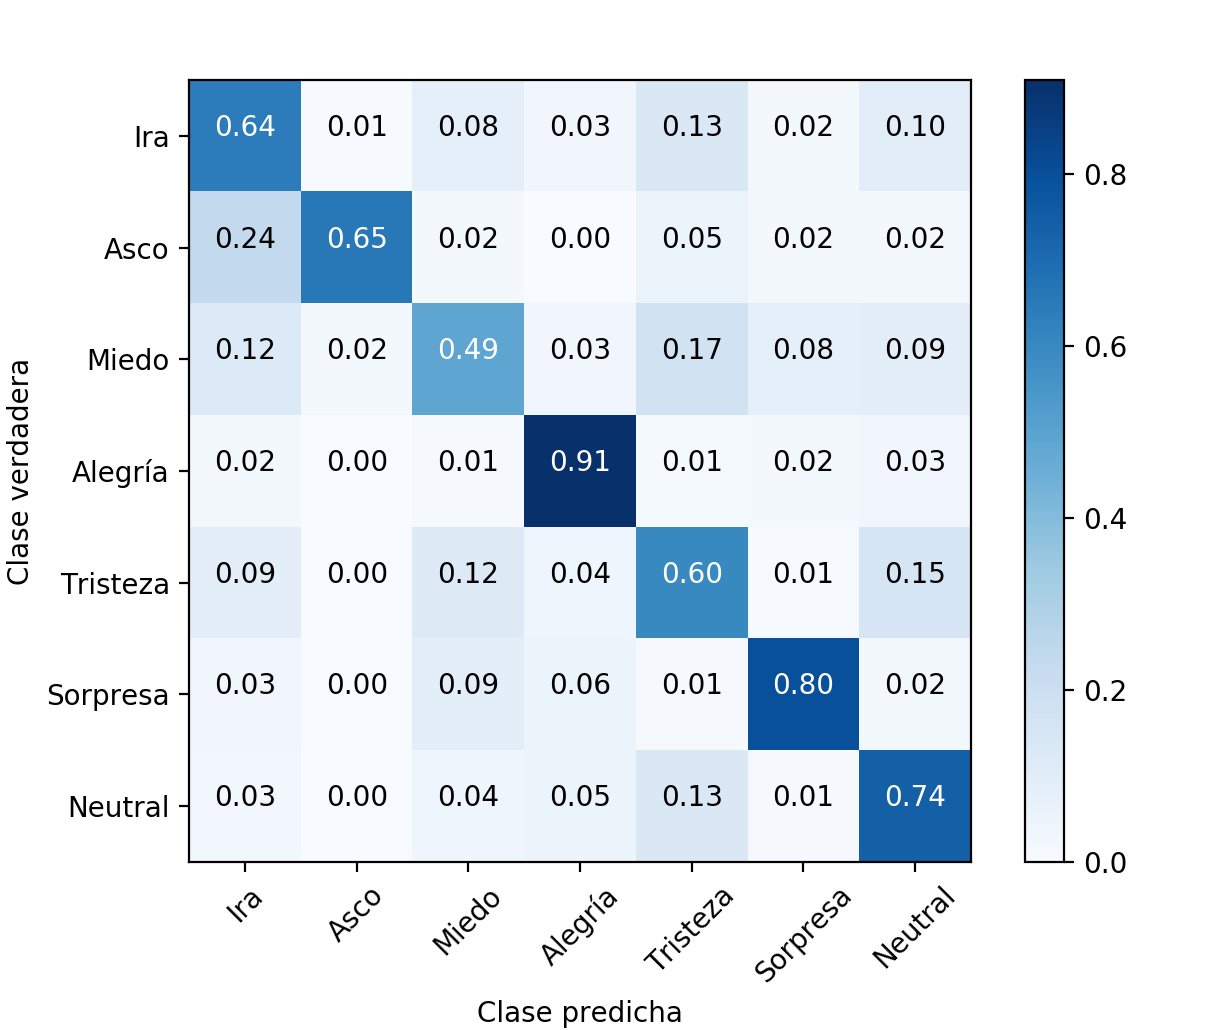
\includegraphics[width=0.7\linewidth]{Images/ResNet-50_matrix_norm.png}
      \caption{Matriz de confusión normalizada del modelo ResNet-50.}
      \label{fig:ResNet-50_matrix_norm}
    \end{subfigure}
    \caption{Matrices de confusión del conjunto de evaluación de la base de datos FER-2013 estimadas sobre el modelo entrenado ResNet-50.}
    \label{fig:ResNet-50_matrices}
\end{figure}

%% CYCLEGAN METRICS

\begin{figure}
    \centering
    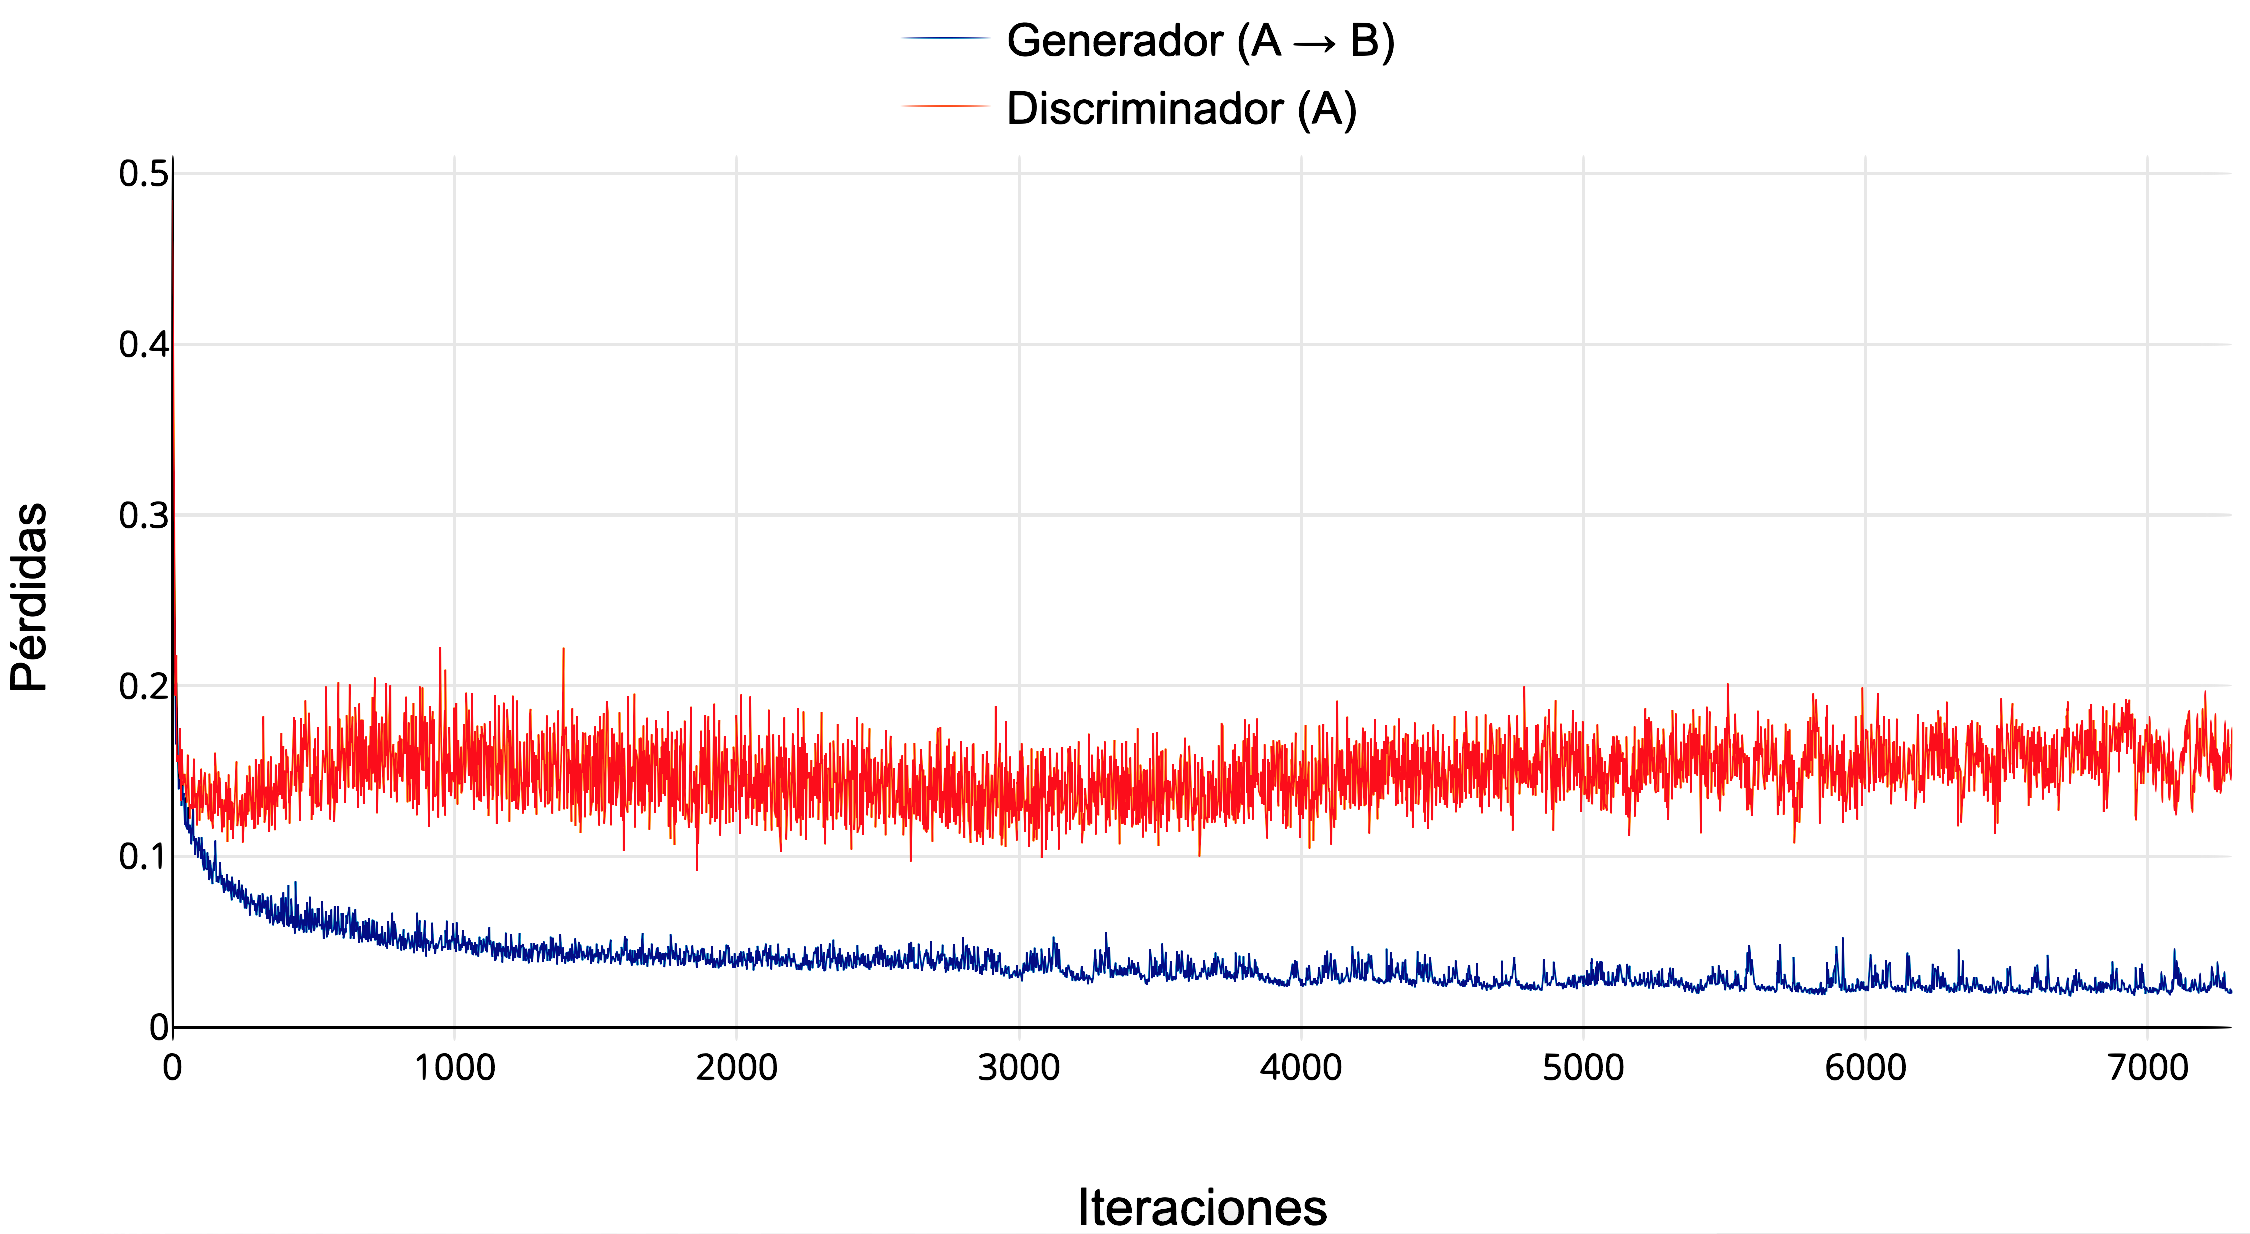
\includegraphics[width=\textwidth]{Images/CycleGAN_metrics.png}
    \caption{Pérdidas del generador $A\rightarrow B$ y del discriminador $A$ de la red CycleGAN (\autoref{fig:CycleGANArchitecture}) a lo largo de su entrenamiento.}
    \label{fig:CycleGAN_metrics}
\end{figure}